\chapter{The Bow}\label{ch:bow}
The bow is an extremely interesting excitation mechanism from a simulation perspective.
A bow excites a string with a force due to friction, which introduces a nonlinear element into the system.
The string `sticks' to the bow and `slips' again when the restoring force of the string is too great and overcomes the friction force. This `stick-slip' behaviour, first coined by Bowden and Leben in 1939 \cite{Bowden1939} causes the string to move in a characteristic triangular motion where the corner of the triangle moves back and forth along the string (see Figure \ref{fig:helmholtz}). Herman Helmholtz was the first to discover this behaviour in the 19\th century, and later got named \textit{Helmholtz motion} in his honour \cite{Helmholtz1860}.\footnote{Also see \url{https://www.youtube.com/watch?v=6JeyiM0YNo4}}

\begin{figure}[h]
    \centering
    \begin{tikzpicture}[->,node distance=3cm,
        thick,main node/.style={circle,draw}, scale=0.96, every node/.style={scale=0.96}]
    
        \node[] (image) at (0,0) {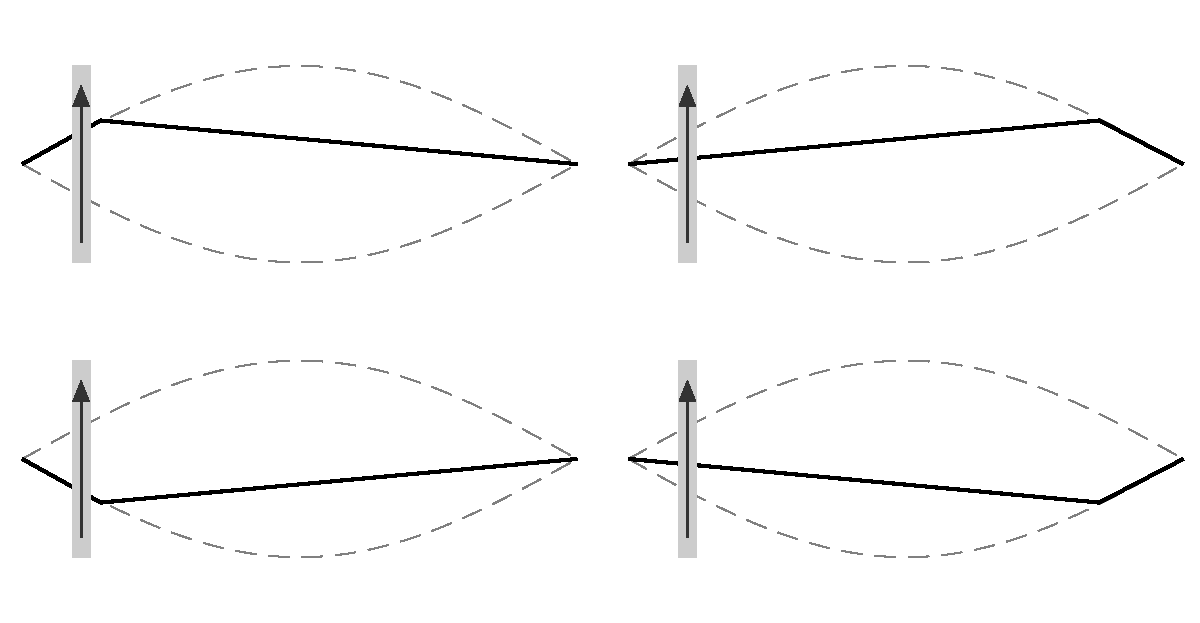
\includegraphics[width=1\columnwidth]{figures/exciters/helmholtz.eps}};
    
        \draw[thick, ->] (-0.25,0.60) arc (110:430:0.6);
        
      \end{tikzpicture}
    \caption{Helmholtz motion. If the bow moves up on the left side of the string, the `Helmholtz corner' travels anti-clockwise. \label{fig:helmholtz}}
\end{figure}

The Helmholtz motion gives bowed string instruments, such as the violin and cello, their characteristic sound. An ideal case is shown in Figure \ref{fig:helmholtzTimedomain}, where, for a string described by $u(x,t)$, the location of a point $x_\text{out}$ along the string follows a sawtooth-like motion due to the `stick-slip' behaviour. 
% Figure \ref{fig:helmholtzImplementation} for a time domain output of one point along a bowed stiff string. The string is bowed upwards, and the `stick-slip' behaviour is visible (stick for upwards, slip for downwards motion), creating a sawtooth pattern. 
\begin{figure}[t]
    \centering
    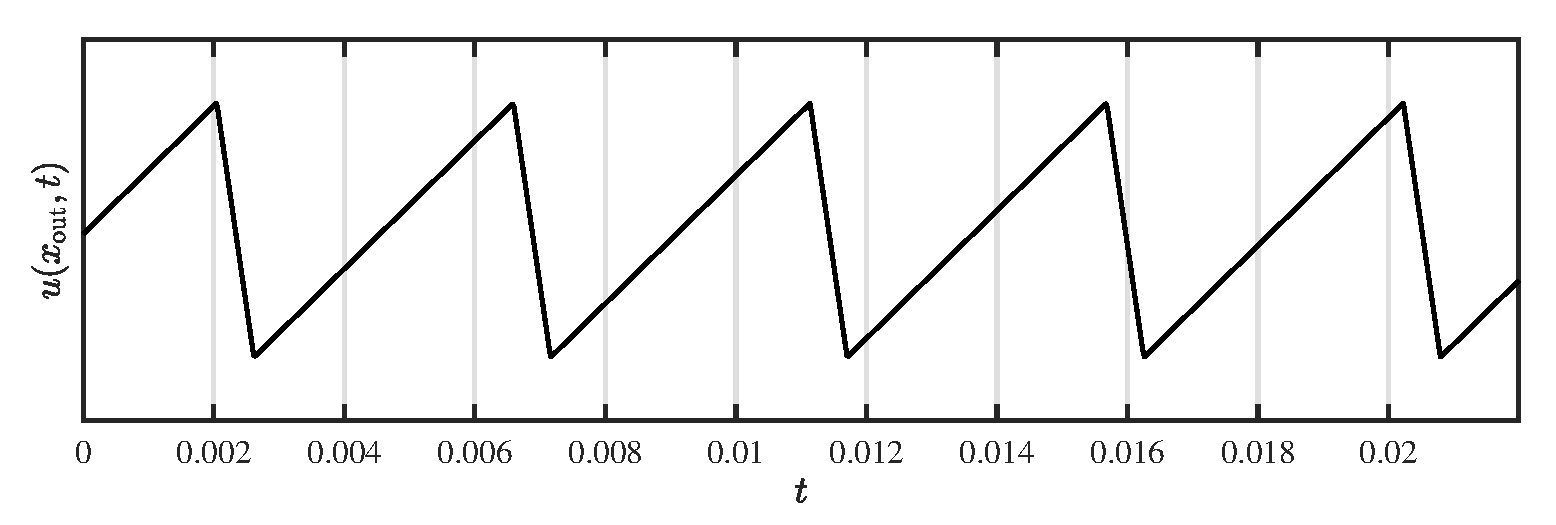
\includegraphics[width=\textwidth]{figures/exciters/helmholtzTimedomain.eps}
    \caption{An example of the (ideal) Helmholtz motion of a location $x_\text{out}$ along a bowed string. \label{fig:helmholtzTimedomain}}
\end{figure}

The rest of this chapter is structured as follows: first, a brief history of bowed-string simulations is presented. Then, an introduction to interpolation and spreading operators, as well as an introduction to the Newton-Raphson method will be given, both of which are necessary to work with bow-string interaction. Finally, a static and a dynamic friction model are presented. The latter, the elasto-plastic friction model, was applied to a FD scheme of the stiff string during this project and is one of the contributions, published in paper \citeP[C].

\section{Brief history of bowed-string simulation}
The first nonlinear systems in the context of musical instrument simulations, including the bowed string, were presented by McIntyre, et al. in 1983 \cite{McIntyre1983}. The first real-time implementation of the bowed string was due to Smith in 1986 and used digital waveguides for the string and a look-up table for the friction model \cite{Smith1986}. Simultaneously, Florens et al. presented a real-time implementation of the bowed string, but instead, the string was modelled using mass-spring systems and the friction model used a static friction model \cite{Florens1986} (see Section \ref{sec:staticFricMod}). One of the most complex friction models applied in a musical context to-date is the elasto-plastic friction model due to Dupont \cite{Dupont2002}, which Serafin et al. \cite{Serafin2003, Serafin2004} applied to a digital waveguide implementation of the string. 

The first appearance of FDTD methods in bowed string simulations was in a publication by Pitteroff and Woodhouse in \cite{Pitteroff1998}. Later, Maestre et al. in \cite{Maestre2014} used FDTD methods to implement a thermal friction model proposed by Woodhouse in \cite{Woodhouse2003}. In both cases, the string was implemented using digital waveguides. Desvages implemented a bowed string model using a static friction model and a two-polarisation FDTD model for the string in \cite{Desvages2016, Desvages2018}, but did not implement this in real-time. The first real-time implementation of a bowed stiff string fully modelled using FDTD methods was presented in paper \citeP[A]. Finally, paper \citeP[C] presented the first (real-time) implementation of the elasto-plastic friction model applied to a FD scheme in a musical context.

\section{Interpolation and spreading operators}\label{sec:interpolationSpreading}
To listen to, or interact with a FD scheme between grid points, it is necessary to use some form of interpolation. 
% As should be clear by now, FD schemes are an approximation to continuous space (and time) using a finite number of points. Working with the system between grid points is not impossible, but requires an extra step. If one would like to listen to a location between specified grid points, one can use interpolation. 
For this end, an \textit{interpolation operator} $I(x_\itxt)$ can be introduced and can be applied to a grid function \cite{theBible}. This operator is a function of $x_\itxt$, the (continuous) location of interest and can be defined in various levels of accuracy. In this section, a 1D system $u(x,t)$ is assumed where $x\in \D$ for spatial domain $\D$. The theory presented in this section will be extended to 2D in Section \ref{sec:interpolationSpreading2D}.

An interpolation operator can be applied to a grid function $\uln$, which performs the following operation:
\begin{equation}
    I_{l,o}(x_\itxt)u_l^n = \sum_{l\in d} I_{l,o}(x_\itxt)\cdot u_l^n.
\end{equation} 
Here, $o$ is the order of the operator, and $l\in d$ with discrete domain $d$, which needs to be the same for both $I_{l,o}(x_\text{i})$ and $\uln$.

The simplest interpolation operator is of '0\textsuperscript{th}'-order and is defined as
\begin{equation}\label{eq:zerothOrderI}
    I_{l,0}(x_\itxt) = \begin{cases}
        1, & \text{if}\ l = l_\itxt,\\
        0, & \text{otherwise},
    \end{cases}
\end{equation}
where the grid location of interest is defined as $l_\itxt = \floor[x_\itxt / h]$ (see Figure \ref{fig:zerothOrderInterpol}). Instead of actually performing an interpolation operation, $I_0$ simply floors its input to the grid location below. 
%As an example, for a 1D system of length $L=1$ described by $u(x,t)$, the location of interest is at $x_\itxt = 0.25$. If the grid spacing $h = 0.2$ the grid point of interest will be $l_\itxt = \floor[0.25/0.2] = \floor[1.25] = 1$. Writing this in operator form yields
% \begin{equation*}
%     u(0.25, t)\approxeq I_{l,0}(0.25)\uln = u_1^n.
% \end{equation*}
%
% \input{exciters/interpolation.tex}
%
A slightly more accurate way to perform 0\thOrder interpolation is to round $x_\itxt/h$ to the nearest neighbour, rather than using the flooring operation. 

First-order or linear interpolation uses the fractional part of the flooring operation as well, according to $\alpha_\itxt = x_\itxt / h - l_\itxt$ and is defined as
\begin{equation}\label{eq:firstOrderI}
    I_{l,1}(x_\itxt) = \begin{cases}
        (1-\alpha_\itxt), & \text{if}\ l = l_\itxt,\\
        \alpha_\itxt , & \text{if}\ l = l_\itxt + 1,\\
        0 & \text{otherwise.}
    \end{cases}
\end{equation}
See Figure \ref{fig:firstOrderInterpol}. 
% Using the same example as before, $\alpha = 1.25 - \floor[1.25] = 0.25$ and
% \begin{equation*}
%     u(0.25, t)\approxeq I_{l,1}(0.25)\uln = 0.75u_1^n + 0.25 u_2^n,
% \end{equation*}

The highest order interpolator used in this project is the Lagrange cubic interpolator: 
\begin{equation}\label{eq:cubicI}
    I_{l,3}(x_\itxt) = \begin{cases}
        -\alpha_\itxt (\alpha_\itxt-1)(\alpha_\itxt-2)/6, & l = l_\itxt-1,\\
        (\alpha_\itxt-1)(\alpha_\itxt+1)(\alpha_\itxt-2)/2,  & l = l_\itxt,\\
        -\alpha_\itxt (\alpha_\itxt+1)(\alpha_\itxt-2)/2, & l = l_\itxt + 1,\\
        \alpha_\itxt (\alpha_\itxt+1)(\alpha_\itxt-1)/6, & l = l_\itxt + 2,\\
        0, & \text{otherwise.}
    \end{cases}
\end{equation}
See Figure \ref{fig:cubicInterpol}. 
% Applied to a grid function using the same example as before, yields
% \begin{equation*}
%     u(0.25, t)\approxeq I_{l,3}(0.25)\uln = -0.0547u_0^n + 0.8203u_1^n + 0.2734u_2^n -0.0391 u_3^n.
% \end{equation*}
Notice that the sum of all values of $I_{l, o}(x_\itxt)$, regardless of the order or the value of $\alpha_\itxt$, add up to $1$.


One could potentially create higher-order interpolation operators, but as one is restricted to a finite domain, the flexibility of the implementation reduces. Notice that if $\alpha_\itxt = 0$, the higher-order interpolators reduce to the $0$\thOrder interpolator in Eq. \eqref{eq:zerothOrderI}.
\def\figWidth{0.32}
\begin{figure}[h]
    \centering
    \subfloat[$0$\thOrder interpolation.\label{fig:zerothOrderInterpol}]{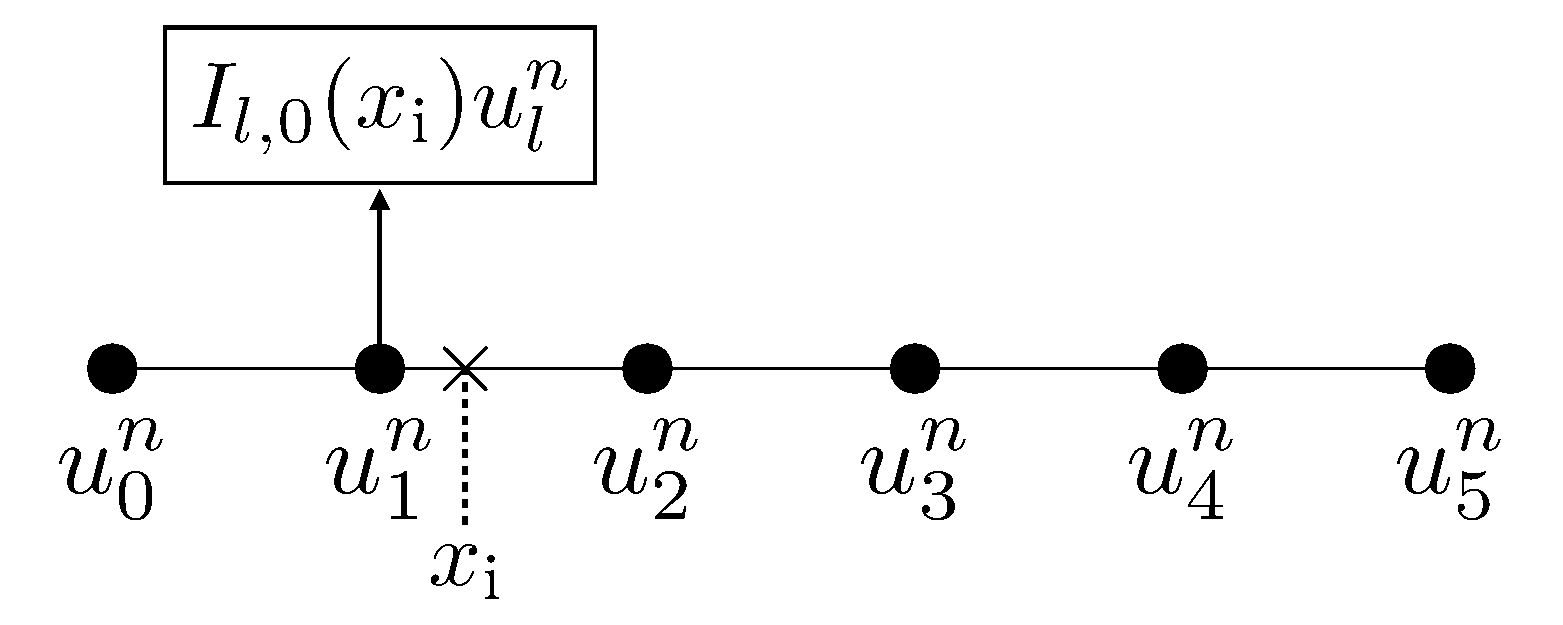
\includegraphics[width=\figWidth\textwidth]{figures/exciters/noInterpol2.pdf}}\hfill
    \subfloat[Linear interpolation.\label{fig:firstOrderInterpol}]{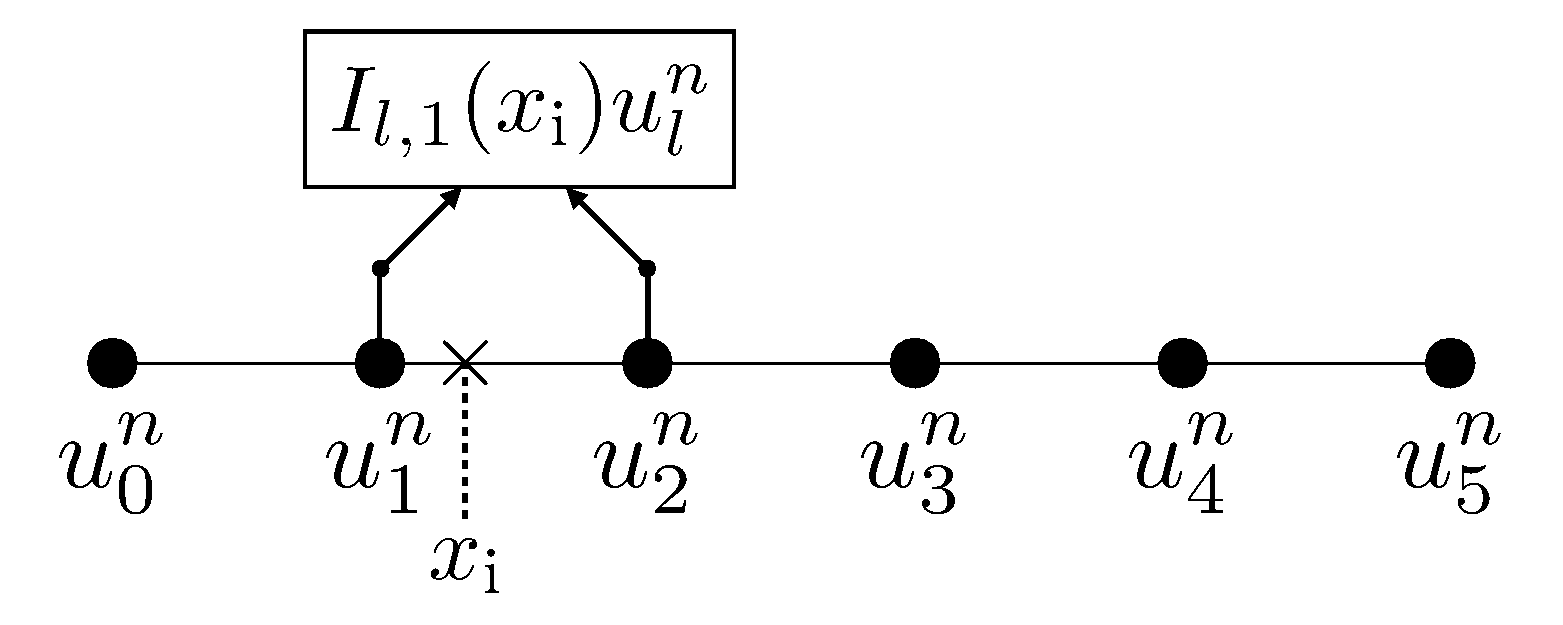
\includegraphics[width=\figWidth\textwidth]{figures/exciters/linearInterpol2.pdf}}\hfill
    \subfloat[Cubic interpolation.\label{fig:cubicInterpol}]{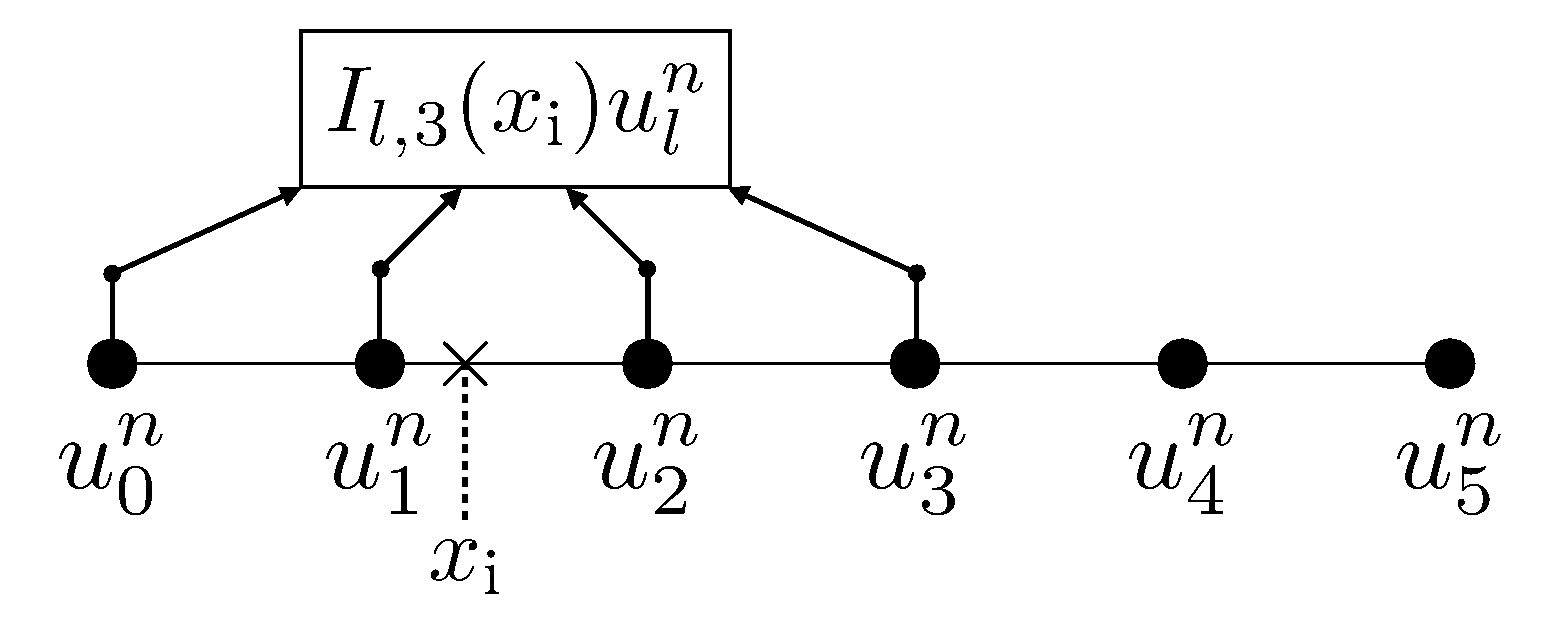
\includegraphics[width=\figWidth\textwidth]{figures/exciters/cubicInterpol2.pdf}}
    \caption{Interpolation with varying orders of accuracy.\label{fig:interpolation}}
\end{figure}

Apart from interpolation operators, one may define \textit{spreading operators} which can be interpreted as an inverse interpolation operation. A spreading operator $J(x_\itxt)$ is used to interact with a distributed FD scheme in the form of an excitation or other interactions such as connections or collisions between multiple schemes (also see Part \ref{part:interactions}).

The spreading operators can be defined in the same way as the interpolation operators described above, yielding a $0$\thOrder spreading operator
\begin{equation}\label{eq:zerothOrderJ}
    J_{l,0}(x_\itxt) = \frac{1}{h}\begin{cases}
        1, & \text{if}\ l = l_\itxt,\\
        0, & \text{otherwise},
    \end{cases}
\end{equation}
a linear spreading operator
\begin{equation}\label{eq:firstOrderJ}
    J_{l,1}(x_\itxt) = \frac{1}{h}\begin{cases}
        (1-\alpha_\itxt), & \text{if}\ l = l_\itxt,\\
        \alpha_\itxt , & \text{if}\ l = l_\itxt + 1,\\
        0 & \text{otherwise,}
    \end{cases}
\end{equation}
and a Lagrange cubic spreading operator
\begin{equation}\label{eq:cubicJ}
    J_{l,3}(x_\itxt) = \frac{1}{h}\begin{cases}
        -\alpha_\itxt (\alpha_\itxt-1)(\alpha_\itxt-2)/6, & l = l_\itxt-1,\\
        (\alpha_\itxt-1)(\alpha_\itxt+1)(\alpha_\itxt-2)/2,  & l = l_\itxt,\\
        -\alpha_\itxt (\alpha_\itxt+1)(\alpha_\itxt-2)/2, & l = l_\itxt + 1,\\
        \alpha_\itxt (\alpha_\itxt+1)(\alpha_\itxt-1)/6, & l = l_\itxt + 2,\\
        0, & \text{otherwise.}
    \end{cases}
\end{equation}
Notice the scaling by $1/h$ which will be more elaborated on in Chapter \ref{ch:connections}. As is the case with the interpolation operators, higher-order spreading operators reduce to Eq. \eqref{eq:zerothOrderJ} if $\alpha_\itxt = 0$.

Spreading operators approximate the spatial Dirac delta function $\delta(x-x_\itxt)$ (in m$^{-1}$), which is a test function defined as
\begin{equation}\label{eq:spatialDirac}
    \delta(x)= \begin{cases}
        \infty, & x = 0,\\
        0, & \text{otherwise},
    \end{cases} \qaq \int_{-\infty}^{\infty} \delta(x)dx = 1,
\end{equation}
used in continuous time to locate an external force to a location $x_\itxt$ along a system distributed over space $x$. Note that the definition in \eqref{eq:spatialDirac} will not be used directly. Instead, it can be approximated using the spreading operators presented in this section. 

\subsubsection{Identities}
The following identity is extremely useful when solving systems including interpolation and spreading operators of the same order $o$ for any (grid) function $f$ and discrete domain $d$:
\begin{equation}\label{eq:identityIJ}
    \langle f_l, J_{l,o}(x_\itxt) \rangle_d = I_{l,o}(x_\itxt) f_l,
\end{equation}
where $l\in d$. From this, it follows that taking the norm of a spreading operator over a given domain is identical to applying to its `dual' interpolation operator (of the same order $o$ and same input $x_\itxt$):
\begin{equation}\label{eq:JnormIJ}
    \langle  J_{l,o}(x_\itxt), J_{l,o}(x_\itxt)\rangle_d = \lVert J_{l,o}(x_\itxt)\rVert^2_d = I_{l,o}(x_\itxt)J_{l,o}(x_\itxt).
\end{equation}
See Section \ref{sec:innerProduct} for more details on the inner product and the norm.

\subsubsection{Other distributions}
This section presented interpolation and spreading operators that interact with the state of a FD scheme at a single location $x_\itxt$ and either interpolates or distributes over a range of points. Although multiple grid points might be used for these operations, the interpolation or spreading is not \textit{distributed}. Physical exciters such as mallets or bows have a non-zero width and thus interact with a larger part of the system. One could make an arbitrary distribution function $E$ with elements $e_l$ (in 1D) where $l\in d$ for discrete domain $d$ of the system at hand. The \textit{distribution} and spreading operators become
\begin{equation}\label{eq:otherDistribution}
    I_l = \frac{e_l}{\sum_d e_l} \qaq J_l = \frac{1}{h}I_l.
\end{equation}
Although any values for $E$ would work, to retain correct scaling, the sum of $E$ needs to be normalised to $1$ as shown in Eq. \eqref{eq:otherDistribution}.

\section{The Newton-Raphson method}\label{sec:newtonRaphson}
Before moving on to more complex nonlinear excitation mechanisms, it is useful to go over the process of how to solve some of these mechanisms using an iterative root-finding method called the \textit{Newton-Raphson} method (or Newton-Raphson for short). 

If a FD scheme not be solved explicitly, due to an implicit dependence on a variable for example, Newton-Raphson can be used. For a continuous and differentiable function $f(x) = 0$, its root can be approached using the following iteration
\begin{equation}\label{eq:newtonRaphson}
    x_{i+1} = x_i - \frac{f(x_i)}{f'(x_i)}\ ,
\end{equation}
with iteration number $i$ and the tick is used to denote a derivation with respect to $x$.
This iteration will then be carried out until the difference between the values of two consecutive iterations is smaller than a given threshold:
\begin{equation}\label{eq:NRthreshold}
    |x_{i+1} - x_i| < \epsilon,
\end{equation} 
where $\epsilon$ is small, but its value depends on the situation at hand. To prevent Newton Raphson from iterating endlessly (if the iteration can not converge), one can put a cap on the number of iterations allowed. 

Preferably, the starting point of the iteration, $x_0$, should be close to the value of where the root is expected to be. This is especially the case for a higher-ordered function with multiple roots (non-uniqueness) or many local variations. 

Algorithm \ref{alg:NR} shows an example of an implementation of Newton-Raphson using $f(x) = e^x -1\ \Rightarrow\ f'(x) = e^x $ and Figure \ref{fig:NR} visualises the iterative algorithm.
\\
\begin{minipage}{\textwidth}
\setlstMAT
\begin{lstlisting}[caption={Example of an implementation of the Newton-Raphson method using $f(x) = e^{x} - 1$.}, label=alg:NR]
% An example of the Newton Raphson method using f(x) = exp(x) - 1

x = 1;          % starting point
eps = 1e-4;     % threshold

% if the threshold has not been crossed before this number of 
% iterations, do not iterate more
maxIterations = 100;    
    
% loop until a maximum number of iterations
for i = 1:maxIterations

    % calculate next iteration (Eq. %*\eqrefMatlab[eq:newtonRaphson]*)
    xNext = x - (exp(x) - 1) / (exp(x));

    % threshold check (Eq. %*\eqrefMatlab[eq:NRthreshold]*)
    if abs(xNext - x) < eps 
        break; % break out of the for loop
    end

    % update the value of x
    x = xNext;
end
disp("The root of f(x) is at x = " + xNext)
\end{lstlisting}
\end{minipage}

\captionsetup[subfigure]{labelformat=empty}
\def\figWidth{0.30}
\begin{figure}[h]
    \centering
    \subfloat[]{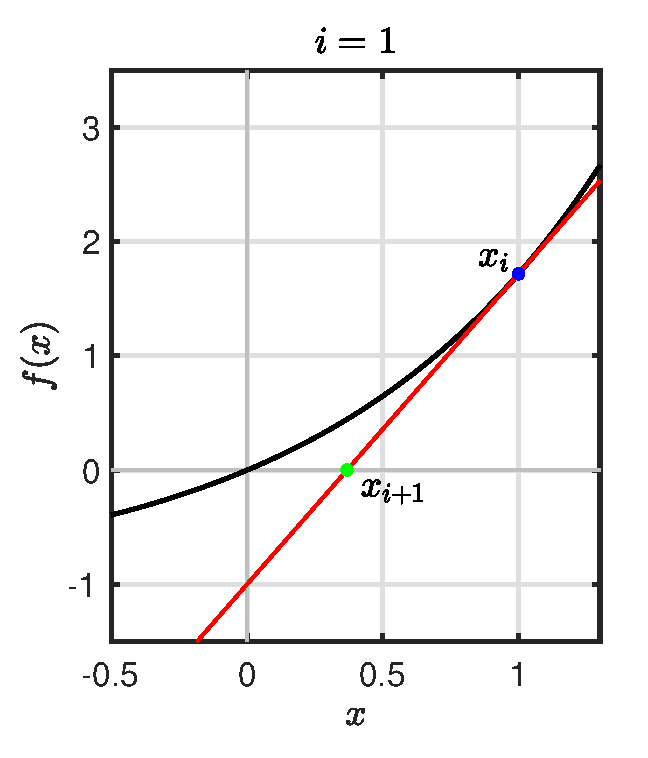
\includegraphics[width=\figWidth\textwidth]{figures/exciters/NR1.eps}}\hfill
    \subfloat[]{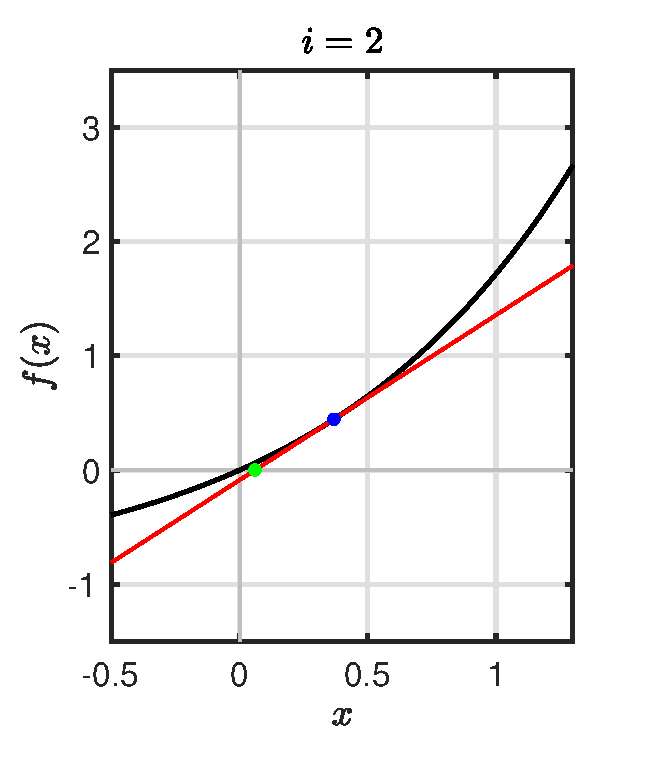
\includegraphics[width=\figWidth\textwidth]{figures/exciters/NR2.eps}}\hfill
    \subfloat[]{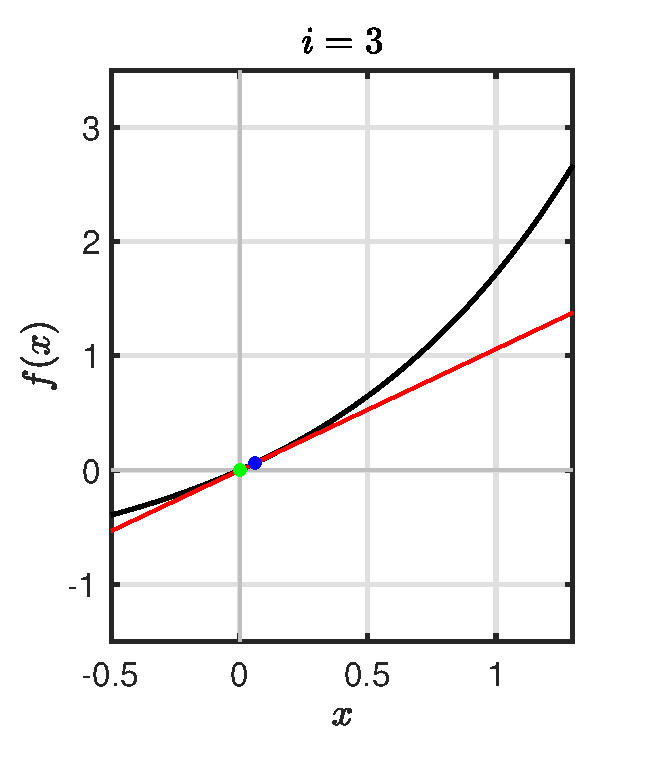
\includegraphics[width=\figWidth\textwidth]{figures/exciters/NR3.eps}}
    \vspace{-2em}\caption{The Newton-Raphson method. The $x$-value of the root of the tangent line at $f(x_i)$ is used to evaluate the next iteration.\label{fig:NR}}
\end{figure}
\captionsetup[subfigure]{labelformat=parens}

\subsection{Multivariate Newton-Raphson}\label{sec:multivariateNR}
For $M$ functions $f_m$ dependent on the same number of independent variables $x_m$ with $m = \{1, \hdots, M\}$, Newton-Raphson can be extended to
\begin{equation}\label{eq:multivariateNR}
    \mathbf{x}_{i+1} = 
    \mathbf{x}_i - 
    {\underbrace{\begin{bmatrix}
        \frac{\partial f_1(\mathbf{x}_i)}{\partial x_1} & \hdots & \frac{\partial f_1(\mathbf{x}_i)}{\partial x_M}\\
        \vdots & \ddots & \vdots\\
        \frac{\partial f_M(\mathbf{x}_i)}{\partial x_1} & \hdots & \frac{\partial f_M(\mathbf{x}_i)}{\partial x_M}
    \end{bmatrix}}_{\mathbf{J}(\mathbf{x}_i)}}^{-1}
    \begin{bmatrix}
        f_1(\mathbf{x}_i)\\
        \vdots\\
        f_M(\mathbf{x}_i)
    \end{bmatrix},
\end{equation}
where the column vector $ \mathbf{x} = [x_1, \hdots, x_M]^T$ is the collection of independent variables, and the iteration number is (again) denoted by $i$.
The matrix in Eq. \eqref{eq:multivariateNR} is referred to as the \textit{Jacobian matrix} $\mathbf{J}$ and contains the derivatives of all functions with respect to each individual independent variable. 

As an example, consider the following system of equations\footnote{Taken from \url{http://fourier.eng.hmc.edu/e176/lectures/NM/node21.html}}:
\begin{subequations}
    \begin{align}
        f_1(\mathbf{x}) &= 3 x_1 - \cos(x_2x_3) - 3/2 = 0,\\
        f_2(\mathbf{x}) &= 4x_1^2 - 625 x_2^2 + 2x_3-1 = 0,\\
        f_3(\mathbf{x}) &= 20 x_3 + e^{-x_1x_2}+9 = 0,
    \end{align} 
\end{subequations}
where $\mathbf{x} = [x_1, x_2, x_3]^T$. The Jacobian matrix will be 
\begin{equation*}
    \mathbf{J}(\mathbf{x}) = \begin{bmatrix}
        3 & x_3 \sin (x_2x_3) & x_2 \sin(x_2x_3)\\
        8x_1 & -1250 x_2 & 2\\
        -x_2e^{-x_1x_2} & -x_1e^{-x_1x_2} & 20
    \end{bmatrix},
\end{equation*}
and its roots can be found by iteratively calculating Eq. \eqref{eq:multivariateNR}.

\section{Static friction models}\label{sec:staticFricMod}
A friction model is a nonlinear function that is (at least) dependent on the relative velocity $\vrel$ between the bow and the string. This function scales how much the bow force affects the bowed object. 
In static friction models, the friction force is defined as a function of this relative velocity only.
The first mathematical description of friction was proposed by Coulomb in 1773 \cite{Coulomb1773}\todo{check references here} to which static friction, or \textit{stiction}, was added by Morin in 1833 \cite{Morin1833} and viscous friction, or velocity-dependent friction, by Reynolds in 1886 \cite{Reynolds1886}. In 1902, Stribeck found a smooth transition between the static and the coulomb part of the friction curve now referred to as the Stribeck effect \cite{Stribeck1902}. The latter is still the standard for static friction models today.

Many static friction models contain a discontinuity where the relative velocity between the  $\vrel = 0$ due to a multiplication with $\sgn(\vrel)$ in their definition. In this project, only the following static friction model has been used \cite{theBible}
\begin{equation}\label{eq:staticFriction}
    \Phi (\vrel) = \sqrt{2a}\vrel e^{-a\vrel^2 + 1/2},
\end{equation}
as it is continuous and differentiable, but still approximating discontinuous bow models. These characteristics make this model easier to work with in implementation. A definition for $\vrel$ will be given below.

\begin{figure}[h]
    \centering
    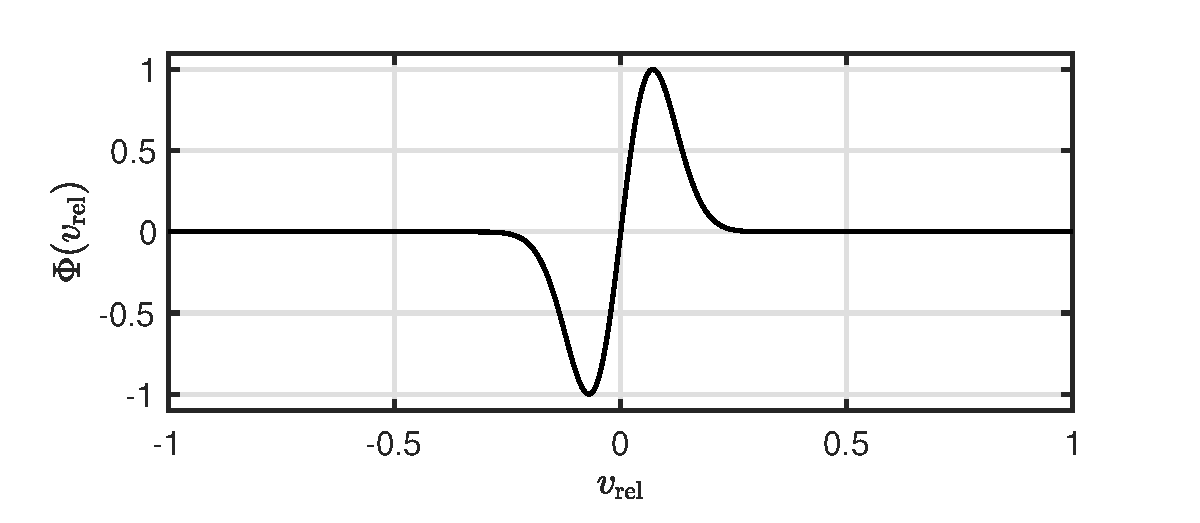
\includegraphics[width=0.8\textwidth]{figures/exciters/frictionCharacteristic.eps}
    \caption{The friction model in Eq. \eqref{eq:staticFriction} with $a = 100$. \label{fig:frictionCharacteristic}}
\end{figure}\todo{FULL DOC SWEEP: check figure centering}
\subsection{The bowed stiff string}\label{sec:bowedStiffStringStatic}
Consider a stiff string, its transverse displacement described by $u(x,t)$ defined for $x\in \D$ (see Chapter \ref{ch:stiffString}). The relative velocity between the string at bow position $x_\Btxt = x_\Btxt(t) \in \D$ and the bow can then be described as
\begin{equation}\label{eq:vrel}
    \vrel = \pt u(x_\Btxt, t) - v_\Btxt(t)
\end{equation}
(in m/s) with bow velocity $v_\Btxt = v_\Btxt(t)$ (in m/s).

Recalling the PDE of the stiff string in Eq. \eqref{eq:stiffStringPDE}
\begin{equation}
    \rho A \ptt u = T \pxx u - EI \pxxxx u - 2 \sz \rho A \pt u + 2 \so \rho A\pt \pxx u,
\end{equation}
one can add the bow force to the equation according to 
\begin{equation}\label{eq:bowedStiffStringPDE}
    \rho A \ptt u = T \pxx u - EI \pxxxx u - 2 \sz \rho A \pt u + 2 \so \rho A\pt \pxx u - \delta(x-x_\Btxt)f_\Btxt\Phi(\vrel)
\end{equation}
where spatial Dirac delta function $\delta(x-x_\Btxt)$ (in m$^{-1}$) (see Section \ref{sec:interpolationSpreading}) positions the bow along the string and $f_\Btxt = f_\Btxt(t) \geq 0$ is the bow force (in N).\footnote{If the spatial Dirac delta function were omitted, the bow force would be applied to the entire string domain rather than only the bow location $x_\text{B}$.} 

\subsubsection{Intuition}
From Eq. \eqref{eq:bowedStiffStringPDE} it can be seen that the bow force gets scaled by the friction model $\Phi(\vrel)$ shown in Figure \ref{fig:frictionCharacteristic}. 
The figure shows that if $\vrel$ is too large (either positively or negatively) the bow term in \eqref{eq:bowedStiffStringPDE} becomes $0$. If, on the other hand, $\vrel$ is closer to $0$, the bow will have an effect on the string. This can be interpreted in terms of static and dynamic friction\footnote{`Static' and `dynamic' friction are unrelated to `static' and `dynamic' friction models.}. A stationary object requires more force to be moved than a moving object, i.e., the static friction coefficient is always higher than the dynamic friction coefficient. This is essentially what the friction model tries to simulate.

It might seem counter-intuitive that the bow term is subtracted from the scheme. This is due to the definition of the relative velocity in Eq. \eqref{eq:vrel}. For a negative bow velocity $v_\Btxt$, $\vrel$ becomes positive. As $\sgn\left(\Phi(\vrel)\right) = \sgn(\vrel)$ through Eq. \eqref{eq:staticFriction} and $f_\Btxt\geq 0$, the term $\delta(x-x_\Btxt)f_\Btxt\Phi(\vrel)$ will be positive for a positive $\vrel$. As a negative $v_\Btxt$ needs to have a downwards, or negative, effect on the string, the sign of the bow term also needs to be negative to achieve this.  

\subsubsection{Discrete time}
Dividing all terms in Eq. \eqref{eq:bowedStiffStringFDS} by $\rho A$ and discretising the system yields
%
\begin{equation}\label{eq:bowedStiffStringFDS}
    \dtt \uln = c^2 \dxx \uln - \kappa^2 \dxxxx \uln - 2 \sz \dtd \uln + 2 \so\dtm\dxx \uln - J_l(x_\Btxt^n)F_\Btxt^n\Phi(\vrel^n),
\end{equation}
with $F_\Btxt^n = f_\Btxt^n/\rho A$ and spreading operator $J_l(x_\Btxt^n) = J_{l,o}(x_\Btxt^n)$ (in m$^{-1}$) as described in Section \ref{sec:interpolationSpreading}, where the order $o$ remains undetermined for now. As the bow position, bow velocity and bow force are time-dependent, these have a superscript $n$ in discrete time. These parameters are called \textit{control parameters} and will be supplied by the performer in an eventual implementation.

The relative velocity in Eq. \eqref{eq:vrel} is discretised using a centred difference operator according to
\begin{equation}\label{eq:vrelDisc}
    \vrel^n = I_l(x_\Btxt^n)\dtd \uln - v_\Btxt^n,
\end{equation}
with interpolation operator $I_l(x_\Btxt^n) = I_{l,o}(x_\Btxt^n)$ and is of the same order as $J_l(x_\Btxt^n)$. Equation \eqref{eq:vrelDisc} makes the scheme implicit due to the centred difference operator as the FD scheme in Eq. \eqref{eq:bowedStiffStringFDS} is now nonlinearly dependent on $u_l^{n+1}$. To solve Eq. \eqref{eq:bowedStiffStringFDS} for $u_l^{n+1}$, an iterative root-finding algorithm, such as Newton-Raphson described in Section \ref{sec:newtonRaphson}, is required. This process could be circumvented by using a backward  difference operator in Eq. \eqref{eq:vrelDisc}, but this will affect the accuracy and behaviour of the bow model.

\subsubsection{Solution}
To find a solution for $u_l^{n+1}$ at the bow location, an inner product of the scheme in Eq. \eqref{eq:bowedStiffStringFDS} with spreading operator $J_l(x_\Btxt^n)$ must be taken over the discrete domain of the string $d$ which isolates the scheme at the bowing location. Performing this operation and using identity \eqref{eq:identityIJ} yields
\begin{equation}\label{eq:bowLocFDS}
    \begin{aligned}
    I_l(x_\Btxt^n)\dtt\uln =\ &c^2 I_l(x_\Btxt^n)\dxx \uln - \kappa^2 I_l(x_\Btxt^n)\dxxxx \uln- 2 \sz I_l(x_\Btxt^n)\dtd \uln\\
    & + 2 \so I_l(x_\Btxt^n)\dtm\dxx \uln - \lVert J_l(x_\Btxt^n)\rVert^2_d F_\Btxt^n\Phi(\vrel^n).
    \end{aligned}
\end{equation}
One can rewrite Eq. \eqref{eq:vrelDisc} to 
\begin{equation}\label{eq:vrelRewritten}
   I_l(x_\Btxt^n)\dtd \uln =  \vrel^n + v_\Btxt^n,
\end{equation}
and using identity \eqref{eq:identity1}, Eq. \eqref{eq:bowLocFDS} can be rewritten and assigned to a function $g(\vrel^n)$ according to 
\begin{equation}\label{eq:staticFrictionNRfunc}
    g(\vrel^n) = \left(\frac{2}{k} + 2\sz\right)\vrel^n + \lVert J_l(x_\Btxt^n)\rVert^2_d F_\Btxt^n\Phi(\vrel^n) + b^n = 0,
\end{equation}
% Here, $b$ contains all terms not dependent on $\vrel$. As the operators can be interchanged, i.e., the order of application does not matter, could write $b$ according to
where the terms not dependent on $\vrel$ are collected in\footnote{An interpolation operator applied to a spatial derivative can be expanded in a similar fashion to when it is applied to a grid function. A first-order interpolator applied to $\dxx \uln$ thus yields $I_{l,1}(x_\itxt) \dxx \uln = (1-\alpha_\itxt)\dxx u_{l_\itxt}^n + \alpha \dxx u_{l_\itxt+1}^n$.}
\begin{equation}\label{eq:staticbDef}
    \begin{aligned}
        b^n =\ &-\frac{2}{k}I_l(x_\Btxt^n)\dtm \uln-c^2 I_l(x_\Btxt^n)\dxx \uln + \kappa^2 I_l(x_\Btxt^n)\dxxxx \uln \\
        &+ \left( \frac{2}{k} + 2 \sz \right)v_\Btxt^n - 2 \so I_l(x_\Btxt^n)\dtm\dxx \uln.
    \end{aligned}
    % b =&\ \left(-\frac{2}{k}\dtm -c^2 \dxx+ \kappa^2\dxxxx - 2 \so \dtm\dxx\right) I(x_\Btxt^n)\uln + \left( \frac{2}{k} + 2 \sz \right)v_\Btxt^n.
\end{equation}
%

One can then perform the Newton-Raphson method detailed in Section \ref{sec:newtonRaphson} to iteratively solve for $\vrel$ 
%
\begin{equation}
    (\vrel^n)_{i+1} = (\vrel^n)_i - \frac{g\left((\vrel^n)_i\right)}{g'\left((\vrel^n)_i\right)}\ ,
\end{equation}
where
\begin{equation*}
    g'(\vrel^n) = \frac{2}{k} + 2\sz + \lVert J_l(x_\Btxt^n)\rVert^2_\D F_\Btxt^n\Phi'(\vrel^n),
\end{equation*}
and 
\begin{equation*}
    \begin{aligned}
        \Phi'(\vrel^n) %&= \sqrt{2a}e^{-a(\vrel^n)^2 + 1/2} + \sqrt{2a}\vrel^n * (-2a\vrel^n)e^{-a(\vrel^n)^2 + 1/2}\\
        %&
        = \sqrt{2a}\left(1 - 2a(\vrel^n)^2\right)e^{-a(\vrel^n)^2+1/2}.
    \end{aligned}
\end{equation*}
\subsection{Implementation and output}\label{sec:staticImplementation}
To implement the bowed stiff string, one must perform the Newton-Raphson iteration every sample. For the implementation shown in this section, the threshold in Eq. \eqref{eq:NRthreshold} has been set to $\epsilon = 10^{-7}$ and the maximum number of iterations to $100$. In the following, the parameters used for the string are listed in Table \ref{tab:stiffStringParams} with $T = 1000$ N and those for the bow are
\begin{equation*}
    x_\Btxt = \floor[0.125/h],\quad f_\Btxt = 1\ \text{N},\quad v_\Btxt = 0.2\  \text{m/s},\qaq a = 100.
\end{equation*}
Figure \ref{fig:staticBowImplementation} shows the behaviour of a bowed stiff string at the beginning of the simulation and shows the characteristic stick-slip behaviour. Figure \ref{fig:helmholtzState} shows the state of the same simulation 3 seconds later. One can observe the Helmholtz corner move in an anti-clockwise direction as presented in Figure \ref{fig:helmholtz}. Finally, the time domain output of the string at the bowing location is shown in Figure \ref{fig:helmholtzImplementation} generally follows the Helmholtz motion shown in Figure \ref{fig:helmholtzTimedomain}. 

\begin{figure}[h]
    \centering
    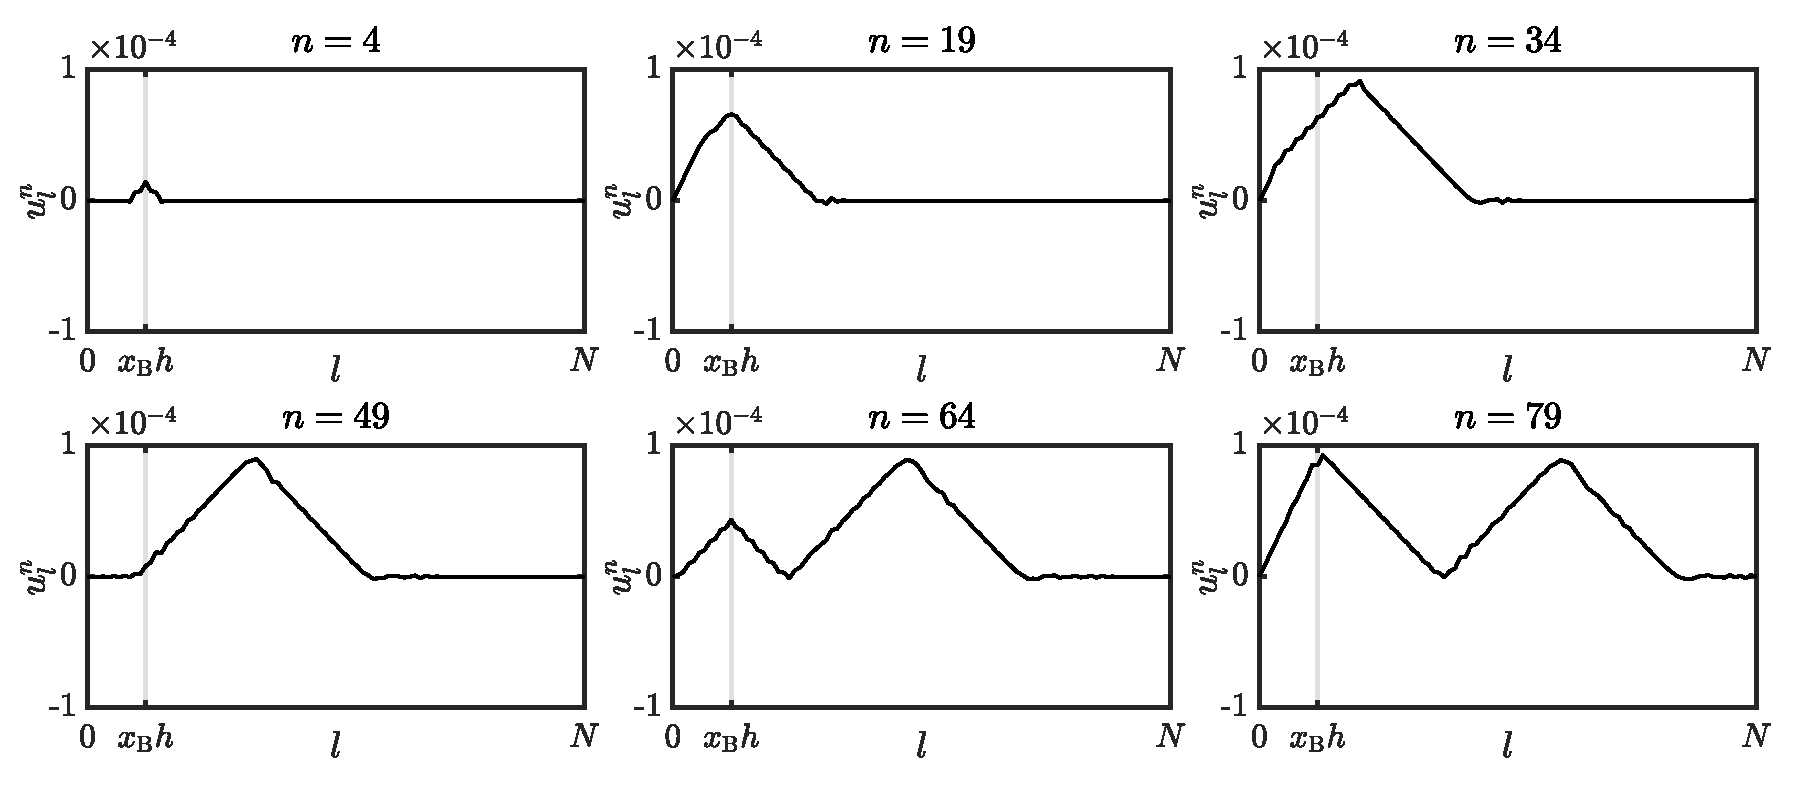
\includegraphics[width=\textwidth]{figures/exciters/bowImplementation.eps}
    \caption{Behaviour of a bowed stiff string at the beginning of the simulation. \label{fig:staticBowImplementation}}
\end{figure}
\begin{figure}[h]
    \centering
    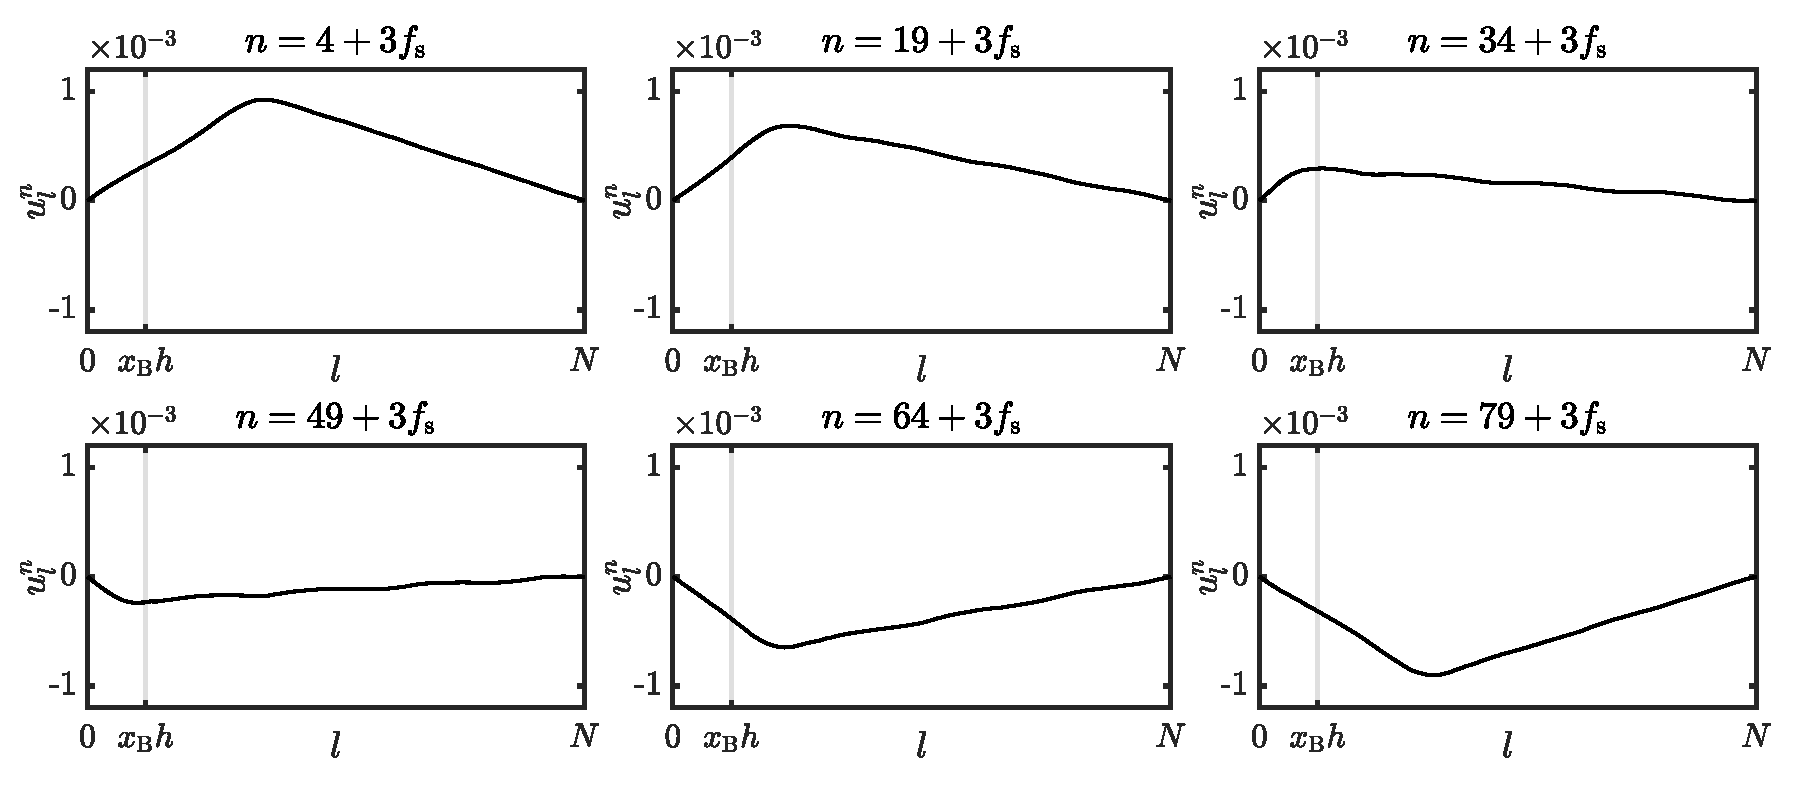
\includegraphics[width=\textwidth]{figures/exciters/helmholtzState.eps}
    \caption{Behaviour of a bowed stiff string simulation after 3 seconds. The string exhibits a Helmholtz motion as presented in Figure \ref{fig:helmholtz}. \label{fig:helmholtzState}}
\end{figure}
\begin{figure}[h]
    \centering
    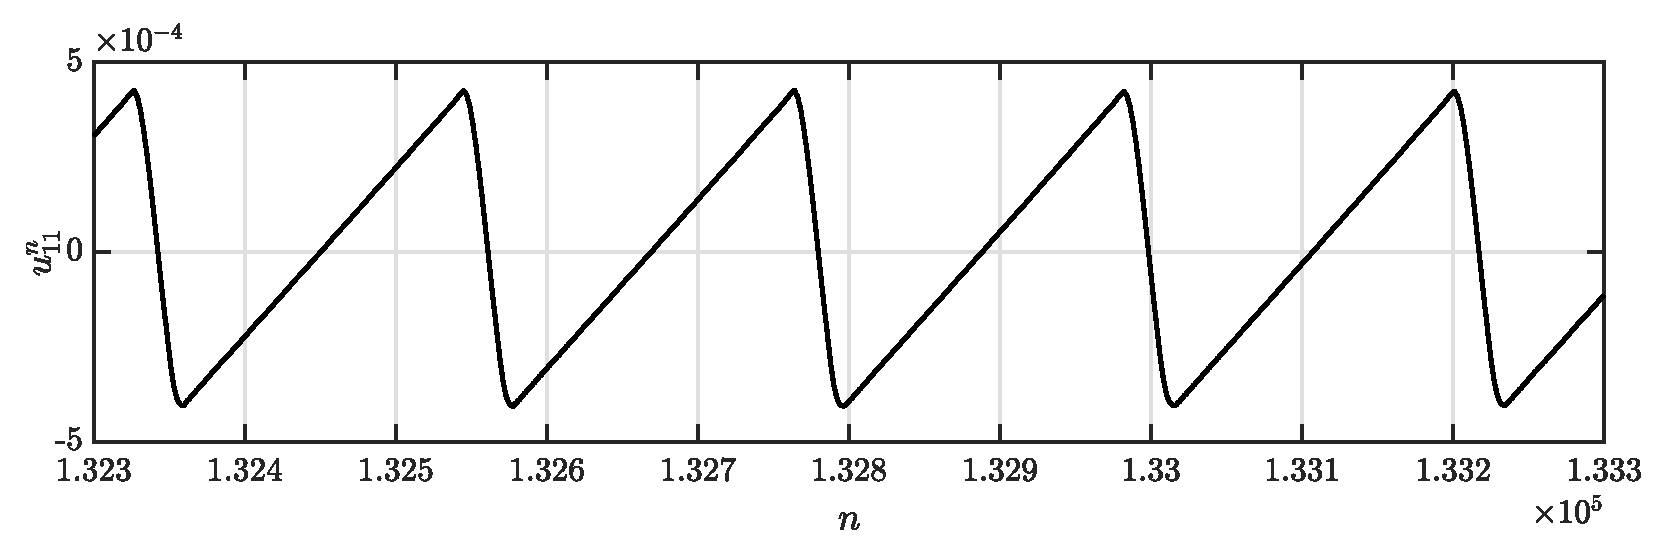
\includegraphics[width=\textwidth]{figures/exciters/helmholtzImplementation.eps}
    \caption{Time domain output at the bowing location of a bowed stiff string using the static friction model in Eq. \eqref{eq:staticFriction}. \label{fig:helmholtzImplementation}}
\end{figure}
\subsection{Energy analysis}
Following the energy analysis of the stiff string presented in Section \ref{sec:energyAnalysisString}, taking an inner product of Eq. \eqref{eq:bowedStiffStringFDS} (after multiplication by $\rho A$) with $(\dtd \uln)$ over discrete domain $d$ one arrives at the following 
\begin{align*}
    \dtp \h + \q &=  - \langle (\dtd \uln), J_l(x_\Btxt^n)f_\Btxt^n\Phi(\vrel^n) \rangle_d\\[-5pt]
    \xLeftrightarrow{\mystrut\ \text{Eq. \eqref{eq:identityIJ}}\ }\qquad &= -I_l(x_\Btxt^n)(\dtd \uln) f_\Btxt^n \Phi(\vrel^n) \\[-5pt]
    \xLeftrightarrow{\mystrut\ \text{Eq. \eqref{eq:vrelRewritten}}\ } \qquad &= \underbrace{-f_\Btxt^n \Phi(\vrel^n) \vrel^n}_{\text{loss}} - \underbrace{f_\Btxt^n \Phi(\vrel^n)v_\Btxt^n}_{\text{power}},
\end{align*}
where $\h$ and $\q$ are as defined in Eqs. \eqref{eq:energyBalanceStiffString} and \eqref{eq:dampingTermStiffString} respectively. As $\sgn\left(\Phi(\vrel^n)\right) = \sgn\left(\vrel^n\right)$ through Eq. \eqref{eq:staticFriction}, one can observe that the first term on the right-hand side always has a negative effect on the rate of change of the total energy. This term can therefore be interpreted as the loss of power through the bow (as indicated). The last term is of indeterminate sign and can thus be interpreted as the power supplied by the bow. 

The final energy balance can thus be written as
\begin{equation}\label{eq:energyBalanceBow}
    \dtp \h = -\q - \q_\text{B} - \p 
\end{equation}
where 
\begin{equation*}
    \q_\text{B} = f_\Btxt^n \Phi(\vrel^n) \vrel^n \qaq \p = f_\Btxt^n \Phi(\vrel^n)v_\Btxt^n.
\end{equation*}
Figure \ref{fig:energyStaticBow} shows the energy of the bowed stiff string corresponding to the wave propagation in Figure \ref{fig:staticBowImplementation}. The bow only injects energy into the system when it sticks to the string. 
% Although the normalised energy shows `jumpy` behaviour, correlated to the behaviour of the system, this decreases for a lower value of $\epsilon$. 

\begin{figure}[h]
    \centering
    \begin{tikzpicture}[->,node distance=3cm,
        thick,main node/.style={circle,draw}]
    
        \node[] (image) at (0,0) {
        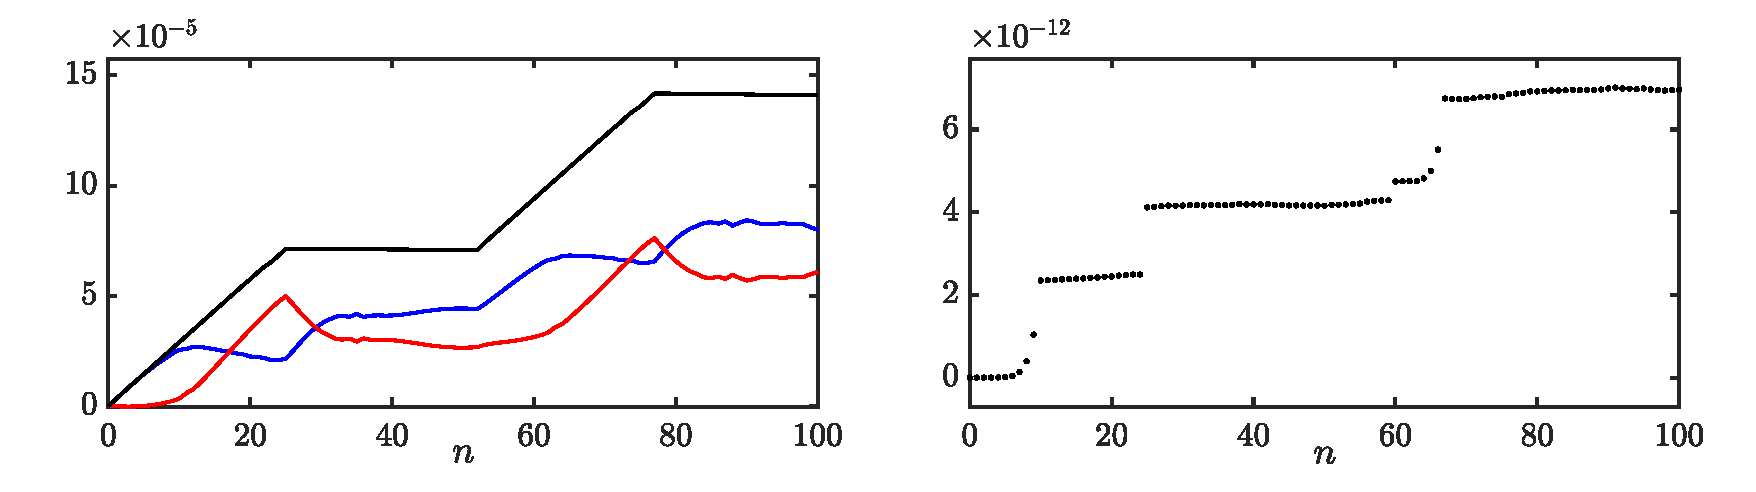
\includegraphics[width=\textwidth]{figures/exciters/energyBow.eps}
        };
    
        \node[] (he) at (0.2,0.5) {\small $\mathfrak{h}_\text{e}$};

        \node[] (h) at (-5.8, 1) {\small $\mathfrak{h}$};
        \node[] (v) at (-5.8, 0.5) {\small $\color{red}\mathfrak{v}$};
        \node[] (t) at (-5.8, 0) {\small $\color{blue}\mathfrak{t}$};
      \end{tikzpicture}
      \caption{The kinetic (blue), potential (red), and total (black) energy of the bowed stiff string. The right panel shows the normalised energy (according to Eq. \eqref{eq:normalisedEnergyDamping}) and shows that the deviation of the energy is within machine precision. \label{fig:energyStaticBow}}
\end{figure}

\section{Dynamic friction models}
As opposed to static friction models, dynamic friction models relate the relative velocity to the friction force using a differential equation. Dynamic friction models exhibit a phenomenon called \textit{hysteresis}, which is the dependence of a system on its history. This hysteresis loop is in the force versus velocity plane and has been confirmed by measurements using a bowing machine in \cite{Woodhouse2003}.

The first dynamic friction model was due to Dahl \cite{Dahl1968} and captured hysteresis effects. The Stribeck effect was, however, not taken into account. The LuGre model (named after the collaboration between Lund and Grenoble) was then proposed by Canudas de Wit et al. in \cite{Canudas1993, Canudas1995} and extended the Dahl model to take the Stribeck effect into account. The model assumes a large ensemble of bristles between the two sliding surfaces, each of which contributes a tiny amount to the total friction force. The drawback of this model is that it exhibits drift for extremely small external forces. In \cite{Dupont2002}, Dupont et al. extended the LuGre model by allowing for a purely elastic regime that solves the drift issue. This model is referred to as the \textit{elasto-plastic} friction model and is used in this project.

\subsection{The elasto-plastic friction model}\label{sec:elastoPlastic}
In a musical context, the elasto-plastic friction has been investigated in-depth by Serafin et al. in \cite{Serafin2003, Serafin2004, Avanzini2005}. Like the LuGre model, the elasto-plastic friction model assumes that the friction between the bow and the string is caused by a large quantity of bristles, all contributing a fraction of the total amount of friction. See Figure \ref{fig:elastoPlastic}.

\begin{figure}[ht]
    \centering
    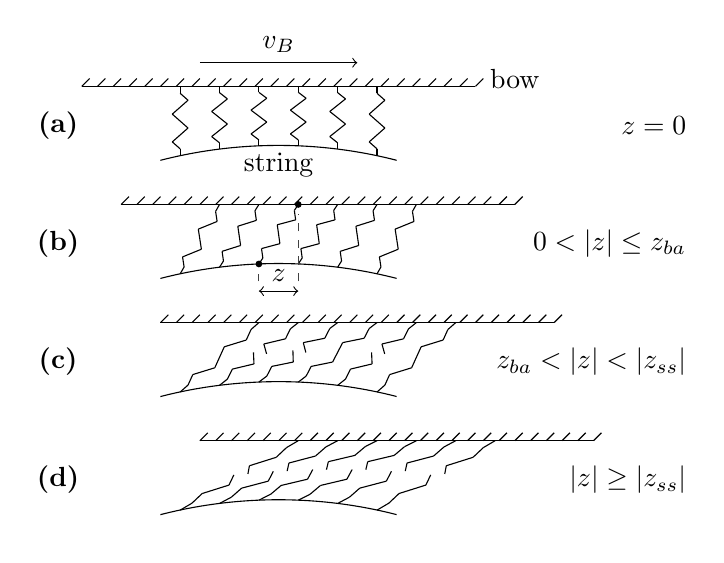
\begin{tikzpicture}
    
    \def\radius{6}; % Radius of the string (>2!)
    \pgfmathsetmacro{\reps}{3}; % How may back-and-forths in the drawing of the springs
    \def\horShift{0.5}; %how far the bow is shifted to the right in b)
    \def\bowSpacing{0.2};
    \def\drawingSpacing{1.5}
    \def\bowWidth{5};
    
    %subfigure letters
    \node (A) at (-2.8, 0.5) {\textbf{(a)}};
    \node (B) at (-2.8, 0.5 - \drawingSpacing) {\textbf{(b)}};
    \node (C) at (-2.8, 0.5 - \drawingSpacing * 2) {\textbf{(c)}};
    \node (D) at (-2.8, 0.5 - \drawingSpacing * 3) {\textbf{(d)}};
    
    %bow velocity arrow
    \draw[->] (-1, 1.3) -- (1, 1.3) node [midway, above] (velText) {$v_\text{B}$};
    
    \pgfmathsetmacro{\zCoordTop}{0};
    \pgfmathsetmacro{\zYCoordBottom}{0};
    \def\springForZ{2}
    \foreach \drawing in {0, ..., 3}
    {
        %% Draw String
        \begin{scope}
            \clip (-1.5,-0.2- \drawing * \drawingSpacing) rectangle (1.5,1.5);
            \draw (0,-\radius + 0.25 - \drawing * \drawingSpacing) circle(\radius);
        \end{scope}

        %% Draw Bow
        \def\halfBW{\bowWidth*0.5}
        \pgfmathsetmacro{\halfNumDiag}{0.5 * \bowWidth / \bowSpacing};
        \draw[-] (-\halfBW + \drawing * \horShift,1 - \drawing * \drawingSpacing) -- (\halfBW + \drawing * \horShift, 1 - \drawing * \drawingSpacing);
        \foreach \bowDiag in {-\halfNumDiag, ...,\halfNumDiag}
        {
        \pgfmathtruncatemacro{\bD}{\bowDiag}
        % \ifnum\drawing=0
        %     \ifnum\bD<-1
        %         \draw[-] (\drawing * \horShift + \bowDiag * \bowSpacing, -\drawing * \drawingSpacing + 1) -- (\drawing * \horShift + \bowDiag * \bowSpacing + 0.1, -\drawing * \drawingSpacing + 0.1 + 1);
        %         \else
        %         \ifnum\bD>1
        %             \draw[-] (\drawing * \horShift + \bowDiag * \bowSpacing, -\drawing * \drawingSpacing + 1) -- (\drawing * \horShift + \bowDiag * \bowSpacing + 0.1, \drawing * -2 + 0.1 + 1);
        %         \fi
        %     \fi
        % \else
            \draw[-] (\drawing * \horShift + \bowDiag * \bowSpacing, -\drawing * \drawingSpacing + 1) -- (\drawing * \horShift + \bowDiag * \bowSpacing + 0.1, -\drawing * \drawingSpacing + 0.1 + 1);
        % \fi
            
        }
        
        \def\brokenSprings{{0, 1, 1, 0, 1, 0}};
        %% Draw Springs
        \foreach \springNo in {0, ..., 5}
        {
            % Calculate spring length depending on the radius of the string
            \pgfmathsetmacro{\startX}{\springNo  * 0.5 - 1.25};
            \pgfmathsetmacro{\calcSpace}{(\radius + 1) - \radius * sin(acos(\startX/\radius)) - 0.25};
            \pgfmathsetmacro{\springLength}{sqrt(\calcSpace*\calcSpace+\drawing*\horShift*\drawing*\horShift)};
            
            \pgfmathsetmacro{\spacing}{\springLength / (\reps + 2)}; 
            % spacing between two spring-back-and-forths
            \ifnum\drawing=0
                \pgfmathsetmacro{\rot}{0};
            \else
                \pgfmathsetmacro{\rot}{(270+(atan(\calcSpace/(\drawing*\horShift))))}; %rotation of the springs
            \fi
            
            \ifnum\drawing=1
                \ifnum\springNo=\springForZ
                    \pgfmathsetmacro{\resTwo}{sqrt(\springLength*\springLength-\horShift*\horShift)};
                    \global\let\zCoordBottom = \resTwo;
                \fi
            \fi
        
            \pgfmathsetmacro{\isBroken}{\brokenSprings[\springNo]};
            % debug code
            % \node (nodeTest\springNo) at (\springNo*1.1-2, -3 - 1 * \drawing + 0.3 * \springNo) {\isBroken};
            
            \begin{scope}[shift={(\startX + \drawing * \horShift,1 -\drawing * \drawingSpacing)}]
                \pgfmathsetmacro{\xWidth}{0.1 - (\drawing * 0.02)};
                \draw[-, rotate = \rot] (0, 0) -- (0, -\spacing * 0.5);
                \draw[-, rotate = \rot] (0, -\spacing * 0.5) -- (\xWidth, -\spacing);
                \def\Y{-\spacing}
                \foreach \idx in {1,...,\reps}
                {
                    \pgfmathsetmacro{\idxMinOne}{\idx-1};
                    \ifnum\drawing=2
                        \ifnum\isBroken=1
                            \pgfmathtruncatemacro{\idxT}{\reps * 0.5 + 1}
                            \ifnum\idx=\idxT
                                \draw[-, rotate = \rot] (\xWidth, \Y - \idxMinOne * \spacing) -- (-\xWidth,\Y - \idx * \spacing*0.6);
                                \draw[-, rotate = \rot] (\xWidth, \Y - \idxMinOne * \spacing * 1.66) -- (-\xWidth,\Y - \idx * \spacing);
                            \else
                                \draw[-, rotate = \rot] (\xWidth, \Y - \idxMinOne * \spacing) -- (-\xWidth,\Y - \idx * \spacing);
                            \fi
                        \else
                                \draw[-, rotate = \rot] (\xWidth, \Y - \idxMinOne * \spacing) -- (-\xWidth,\Y - \idx * \spacing);
                        \fi
                    \else
                        \ifnum\drawing=3
                            \pgfmathtruncatemacro{\idxT}{\reps * 0.5 + 1}
                            \ifnum\idx=\idxT
                                \draw[-, rotate = \rot] (\xWidth, \Y - \idxMinOne * \spacing) -- (-\xWidth,\Y - \idx * \spacing*0.6);
                                \draw[-, rotate = \rot] (\xWidth, \Y - \idxMinOne * \spacing * 1.66) -- (-\xWidth,\Y - \idx * \spacing);
                            \else
                                \draw[-, rotate = \rot] (\xWidth, \Y - \idxMinOne * \spacing) -- (-\xWidth,\Y - \idx * \spacing);
                            \fi
                        \else
                            \draw[-, rotate = \rot] (\xWidth, \Y - \idxMinOne * \spacing) -- (-\xWidth,\Y - \idx * \spacing);
                        \fi
                    \fi
                    \pgfmathsetmacro{\invXWidth}{\xWidth*-1};
                    \global\let\xWidth = \invXWidth;
                    \pgfmathsetmacro{\lastYPre}{\Y - \idx * \spacing};
                    \global\let\lastY = \lastYPre;
                }
                \draw[-, rotate = \rot] (\xWidth, \lastY) -- (0, \lastY - \spacing * 0.5);
                \draw[-, rotate = \rot] (0, \lastY - \spacing * 0.5) -- (0, \lastY - \spacing);
             \end{scope}
             
        }
        % \draw[<->] (2,2-0.707) -- node[right] {$r=\sqrt{2} \Rightarrow A=\pi(\sqrt{2})^2=2\pi$} (2,2+0.707);
        
        % \node(stringText) at (0, -\drawing * 2) {string};
        % \node[block, minimum height = 0.15cm, fill=white, draw=white] (bowText) at (\drawing * \horShift, 1.23 - \drawing * 2) {bow};
    }
    \filldraw[black] (-1.25+\springForZ*0.5 + \horShift,1-\drawingSpacing) circle (1pt) node[anchor=center](topZ){};
    \filldraw[black] (-1.25++\springForZ*0.5,1-\zCoordBottom-\drawingSpacing) circle (1pt) node[anchor=center](bottomZ){};
    
    \node [](leftNode) at (-1.25+\springForZ*0.5,-\drawingSpacing - 0.1) {};
    \node [](rightNode) at (-1.25 +\springForZ*0.5 + \horShift,-\drawingSpacing - 0.1) {};
    
    \draw[<->] (leftNode.center) -- (rightNode.center) node [midway, above] (TextNode) {$z$};
    \draw[dashed, darkgray] (leftNode) -- (bottomZ);
    \draw[dashed, darkgray] (rightNode) -- (topZ);
    %% Draw bow and string texts
        \node(stringText) at (0, 0) {string};
        \node(bowText) at (3, 1.1) {bow};
    %% Draw descriptions of z
    \def\zTexts{{"$z=0$", "$0<|z|<z_{\text{ba}}$", "$z_{\text{ba}}<|z|< z_\text{ss}$", "$|z|>z_\text{ss}$"}};
    
    \node[anchor = east](zText1) at (5.3, 0.5) {$z=0$};
    \node[anchor = east](zText1) at (5.3, 0.5 - \drawingSpacing) {$0<|z|\leq z_{\text{ba}}$};
    \node[anchor = east](zText1) at (5.3, 0.5 - \drawingSpacing * 2) {$z_{\text{ba}}<|z|< |z_\text{ss}|$};
    \node[anchor = east](zText1) at (5.3, 0.5 - \drawingSpacing * 3) {$|z|\geq|z_\text{ss}|$};
    
    \end{tikzpicture}
    \caption{Microscopic displacements of the bristles between the bow and the string. The bow moves right with a velocity of $v_\text{B}$. (a) The initial state is where the average bristle displacement $z=0$. (b) The bow has moved right relative to the string. The purely elastic, or presliding regime is entered (stick). (c) After the break-away displacement $z_\text{ba}$, more and more bristles start to `break'. This is defined as the elasto-plastic regime. (d) After all bristles have `broken', the steady state (slip) is reached and the purely plastic regime is entered. (Adapted from paper \citeP[C].)\SWcomment[exactly the same caption as paper]}
    \label{fig:elastoPlastic}
\end{figure}

Unless denoted otherwise, this section follows the original model by Dupont et al. in \cite{Dupont2002}, but with the appropriate corrections added as presented in paper \citeP[C]. As opposed to the static friction model described in the previous section, the friction force $f$ (in N) is now dependent on the average bristle displacement $z = z(t)$ (in m) as well as the relative velocity $v = v(t)$ (in m/s). The friction force is defined as
\begin{equation}\label{eq:elastoPlasticForce}
    f(v, z) = s_0z + s_1\dot z + s_2v + s_3w,
\end{equation}
with bristle stiffness $s_0 \geq 0$ (in N/m), bristle damping $s_1 \geq 0$ (in kg/s), viscous friction $s_2 \geq 0$ (in kg/s) and, as presented in \cite{Serafin2004}, a dimensionless noise coefficient $s_3$ multiplied onto a pseudorandom function $w = w(t)$ (in N) generating values between $-1$ and $1$. Moreover, for a string defined over domain $\D$, the relative velocity between the string at bowing location $x_\Btxt = x_\Btxt(t) \in \D$ and the bow is (similar to Eq. \eqref{eq:vrel})
\begin{equation}\label{eq:vrelElasto}
    v = \pt u(x_\Btxt,t) - v_\Btxt,
\end{equation}
with bow velocity $v_\Btxt = v_\Btxt(t)$ (in m/s). Lastly, $\dot z$ is the rate of change of the bristle displacement (in m/s) and is related to $v$ according to
\begin{equation}\label{eq:zdot}
    \dot z = r(v, z) = v \bigg[ 1-  \alpha(v, z)\frac{z}{z_\text{ss}(v)}\bigg].
\end{equation}
Here, $z_\text{ss}$ is the steady-state function
\begin{equation}\label{eq:zss}
    z_\text{ss}(v) = \frac{\sgn(v)}{s_0}\left[f_\text{C}+(f_\text{S}-f_\text{C})e^{-(v/v_\text{S})^2}\right],
\end{equation}
where the $v_\text{S}$ is the Stribeck velocity (in m/s). Furthermore, using the normal force $f_\text{N} = f_\text{N}(t)$ (in N), the Coulomb force and stiction force can be calculated according to $f_\text{C} = f_\text{N}\mu_\text{C}$ and $f_\text{S} = f_\text{N}\mu_\text{S}$ respectively (both in N). In these definitions $\mu_\text{C}$ and $\mu_\text{S}$ are the dimensionless dynamic and static friction coefficients respectively. A plot of the steady state function can be found in Figure \ref{fig:zss}.

\begin{figure}[ht]
    \centering
    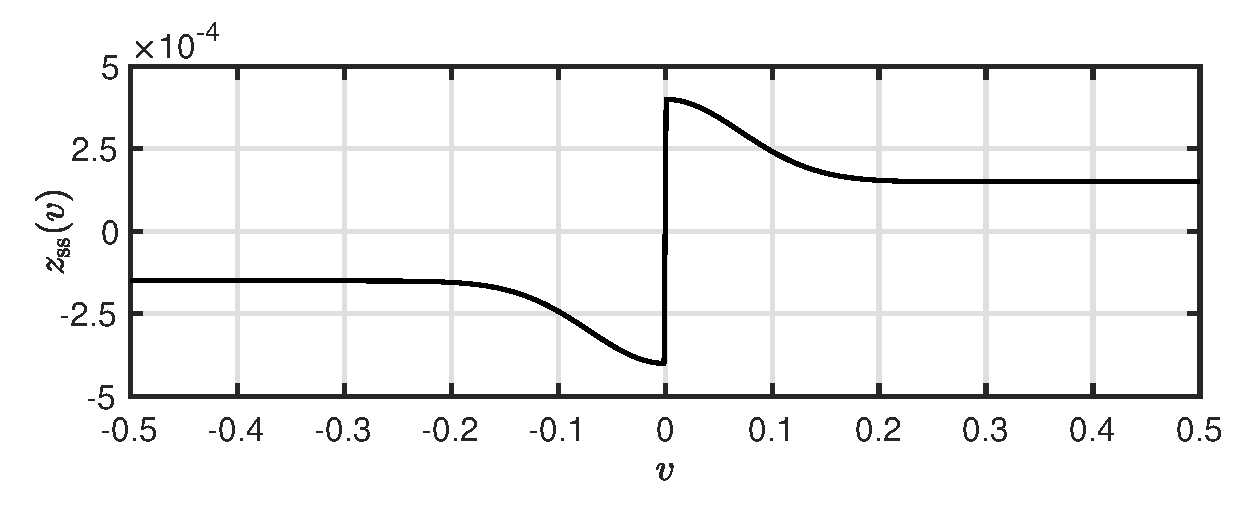
\includegraphics[width=0.8\textwidth]{figures/exciters/steadyState.eps}
    \caption{\label{fig:zss}The steady-state function $z_\text{ss}(v)$ plotted against relative velocity $v$ with $s_0 = 10^4$, $\mu_\text{C} = 0.3$, $\mu_\text{S} = 0.8$, $v_\text{S} = 0.1$ and $f_\text{N} = 5$.}
\end{figure}

Finally, $\alpha(v,z)$ in Eq. \eqref{eq:zdot} is an adhesion map between the bow and the string and is defined as

\begin{equation}\label{eq:adhesionMap}
\alpha(v, z) = 
\begin{aligned}
    \begin{cases}
    \begin{rightcases}
        &0 & |z| \leq z_\text{ba}\\
        &\alpha_\text{m}(v,z)&\ \ \ \, z_\text{ba}<|z|<|z_\text{ss}(v)|\\        &1 &|z|\geq|z_\text{ss}(v)|
        \end{rightcases} 
        
        &\text{if}\  \sgn(v)=\sgn(z)\\
        \,0&\!\,\text{if}\  \sgn(v)\neq\sgn(z),
    \end{cases}
    \end{aligned}
\end{equation}
where the transition between the elastic and plastic behaviour is defined as
\begin{equation}\label{eq:alphaM}
    \alpha_\text{m} = \frac{1}{2}\bigg[1+\sgn(z)\sin\bigg(\pi\frac{z-\sgn(z)\frac{1}{2}(|z_\text{ss}(v)|+z_\text{ba})}{|z_\text{ss}(v)|-z_\text{ba}}\bigg)\bigg],
\end{equation}
where the break-away displacement $z_\text{ba} = z_\text{ba}(t) = 0.7 f_\text{C}/s_0$ determines the value of $z$ before bristles start to break. The adhesion map is visualised in Figure \ref{fig:alphaPlot} and relates to Figure \ref{fig:elastoPlastic} as described in its caption.
\begin{figure}[ht]
    \centering
    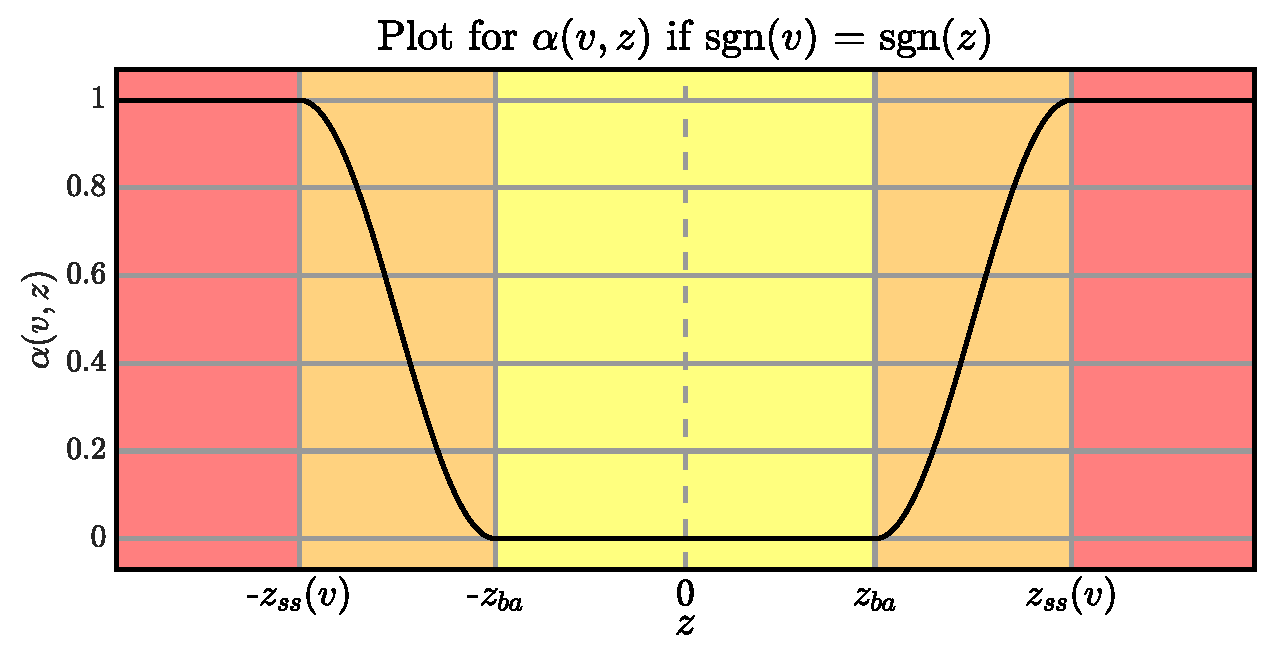
\includegraphics[width=0.8\textwidth]{figures/exciters/drawAlpha3.eps}
    \caption{\label{fig:alphaPlot}A plot of the adhesion map $\alpha(v,z)$ in Eq. \eqref{eq:adhesionMap} plotted against $z$ when $\sgn(v)  = \sgn(z)$. The different coloured regions correspond to Figure \ref{fig:elastoPlastic} according to: yellow - a) \& b), orange - c) and red - d). (Adapted from paper \citeP[C].)}
\end{figure}

\subsubsection{Discrete time}
Equation \eqref{eq:elastoPlasticForce} can be discretised to
\begin{equation}\label{eq:discForceFunction}
    f(v^n,z^n) = s_0z^n + s_1r^n+s_2v^n+s_3w^n
\end{equation} 
where Eq. \eqref{eq:vrelElasto} can be discretised to
\begin{equation}\label{eq:vrelElastoDisc}
    v^n = I_l(x_\Btxt^n)\dtd\uln - v_\Btxt^n,
\end{equation}
with interpolation operator $I_l(x_\Btxt^n) = I_{l,o}(x_\Btxt^n)$ (of unspecified order $o$) and
\begin{equation}\label{eq:r}
    r^n = r(v^n,z^n) = v^n\bigg[1-\alpha(v^n,z^n)\frac{z^n}{z_\text{ss}(v^n)}\bigg]
\end{equation}
is the discrete counterpart of Eq. \eqref{eq:zdot}. The discrete adhesion map is identical to the continuous definition given in Eqs. \eqref{eq:adhesionMap} and \eqref{eq:alphaM}, but with superscripts $n$ added for appearances of $v$ and $z$.

\subsection{Applied to a FDTD stiff string}
The first appearance of a contribution in this work is the elasto-plastic friction model applied to a stiff string implemented using FDTD methods. This has been presented in paper \citeP[C] and will be summarised in this section. \todo{state the stability stuff here?}

In the same way as done with the static friction model in Section \ref{sec:staticFricMod}, one can add the friction force to the stiff string PDE in Eq. \eqref{eq:stiffStringPDE} and discretise the system as follows:
%
\begin{equation}\label{eq:elastoStiffStringFDS}
    \dtt \uln = c^2 \dxx \uln - \kappa^2 \dxxxx \uln - 2 \sz \dtd \uln + 2 \so\dtm\dxx \uln - J_l(x_\Btxt^n)\frac{f(v^n,z^n)}{\rho A},
\end{equation}
where spreading operator $J_l(x_\Btxt^n) = J_{l,o}(x_\Btxt^n)$ and is of the same order as $I_l(x_\Btxt^n)$ in Eq. \eqref{eq:vrelElastoDisc}. Following the same procedure as for the static friction model in Section \ref{sec:staticFricMod}, one takes an inner product with $J_l(x_\Btxt^n)$ over discrete string domain $d$ and using identities \eqref{eq:identityIJ} and \eqref{eq:identity1}, one can rewrite this similar to the static friction model in Eq. \eqref{eq:staticFrictionNRfunc} as
%
\begin{equation}\label{eq:elastog1}
    g_1(v^n,z^n) = \left(\frac{2}{k} + 2\sz\right)v^n + \lVert J_l(x_\Btxt^n)\rVert_d^2\frac{f(v^n,z^n)}{\rho A}+ b^n= 0,
\end{equation}
where
\begin{align*}
    b^n =&-\frac{2}{k}I_l(x_\text{B}^n)\delta_{t-}u_l^n - c^2 I_l(x_\text{B}^n)\delta_{xx} u_l^n +\kappa^2I_l(x_\text{B}^n)\delta_{xxxx} u_l^n\\
    &+\left(\frac{2}{k}+ 2\sigma_0\right)v_\text{B}^n-2\sigma_1I_l(x_\text{B}^n)\delta_{t-}\delta_{xx}u_l^n.
\end{align*}
As $g_1$ contains two unknown variables $v^n$ and $z^n$ that need to be solved for, the multivariate Newton-Raphson method presented in \ref{sec:multivariateNR} must be performed. To be able to do this, an extra function must be included. 

As $r$ describes $\dot z$ in Eq. \eqref{eq:zdot}, one can take another approach to approximate $\dot z$ using the trapezoid rule \cite{theBible}
\begin{equation}
    a^n = (\mtm)^{-1}\dtm z^n \quad \Longrightarrow\quad a^n = \frac{2}{k}(z^n - z^{n-1}) + a^{n-1}.
\end{equation}
As both $a^n$ and $r^n$ approximate $\dot z$, these can be used to create the second function necessary to solve the full system
\begin{equation}\label{eq:elastog2}
    g_2(v^n, z^n) = r^n - a^n = 0.
\end{equation}
Finally, one can use the multivariate Newton-Raphson method described in Section \ref{sec:multivariateNR}, which results in
\begin{equation}\label{eq:NRit}
    \begin{bmatrix}
    v^n\\
    z^n
    \end{bmatrix}_{i+1}
    =
    \begin{bmatrix}
    v^n\\
    z^n
    \end{bmatrix}_i
    -
    \begin{bmatrix}
    \frac{\partial g_1}{\partial v} & \frac{\partial g_1}{\partial z}\\
    \frac{\partial g_2}{\partial v} & \frac{\partial g_2}{\partial z}\\
    \end{bmatrix}^{-1}
    \begin{bmatrix}
    g_1\\
    g_2
    \end{bmatrix}\,
    .
\end{equation}
The derivatives in the Jacobian matrix are given in Appendix \ref{app:elastoDeriv}.

\subsection{Output}
In the following, the same parameters as presented for the static friction model in Section \ref{sec:staticImplementation} have been used for the string and the bow (where $f_N = f_\Btxt$).
Additional parameters used for the elasto-plastic friction model are given in paper \citeP[C].

Figure \ref{fig:hysteresis} shows that the implementation of the elasto-plastic friction model exhibits a hysteresis loop in the force versus velocity plane as desired from a dynamic friction model. The values around $v=0$ are due to sticking behaviour and the loop on the left is due to slipping behaviour.
Figure \ref{fig:elastoWaveform} shows the output of the implementation and follows the characteristic Helmholtz motion shown in Figure 
\ref{fig:helmholtzTimedomain}. When compared to the output of the static friction model in Figure \ref{fig:helmholtzImplementation}, the output of the elasto-plastic implementation seems to be more `smooth' overall, which could be explained by the elasticity of the bristles. 

\begin{figure}[ht]
    \centering
    \begin{tikzpicture}[->,node distance=3cm,
      thick,main node/.style={circle,draw}, scale=0.9, every node/.style={scale=0.9}]
  
      \node[anchor=south west,inner sep=0] (image) at (0,0) {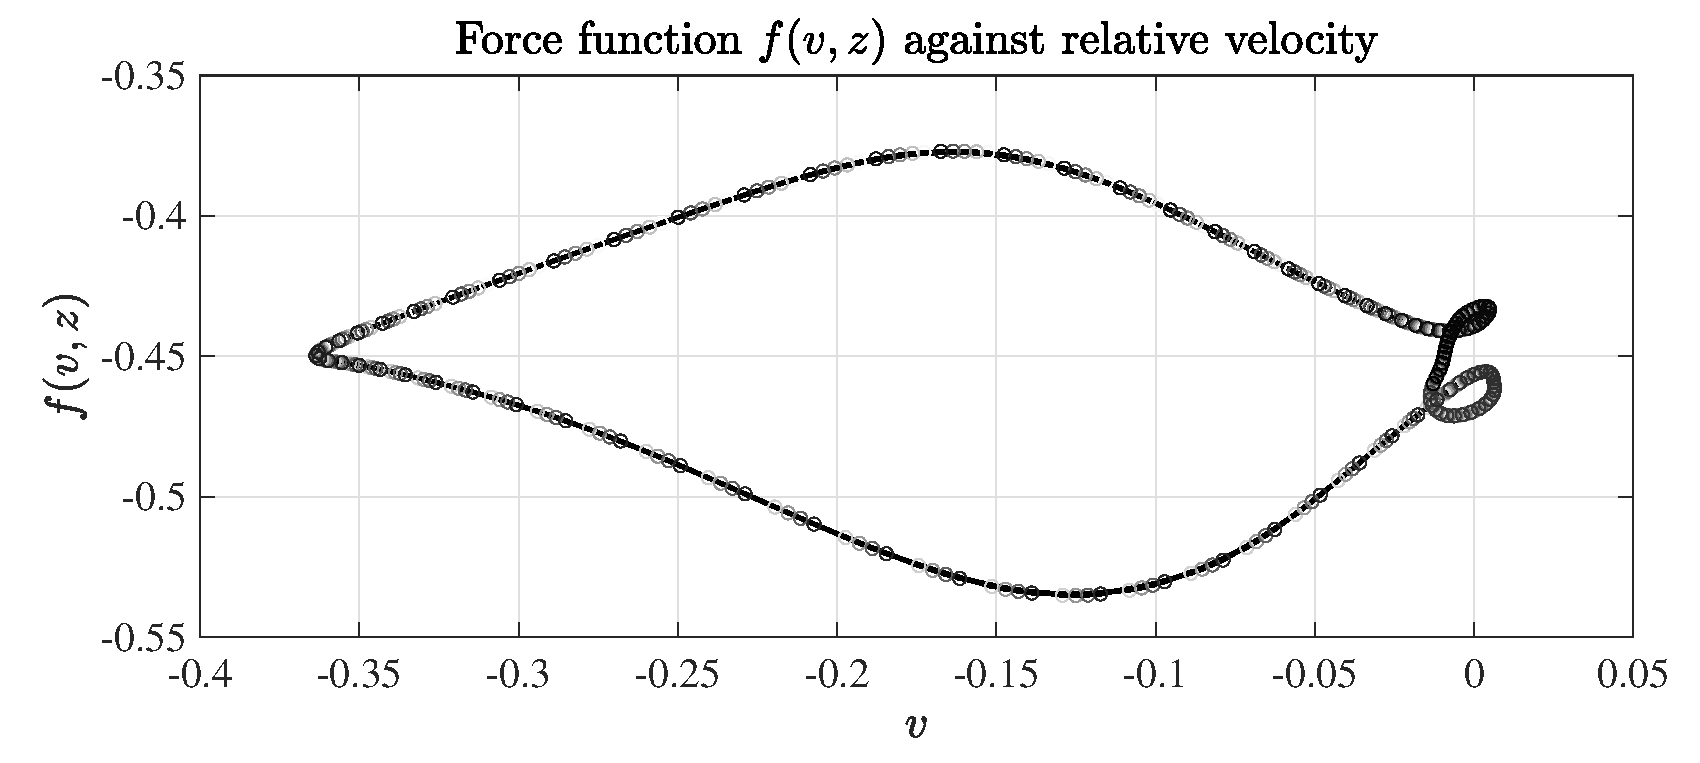
\includegraphics[width=\textwidth]{figures/exciters/hysteresis.eps}};
      % \filldraw[black] (arr2B) (2,2) circle (1pt) node[anchor=center](topZ){};
      % \filldraw[black] (arr2E) (3,1.5) circle (1pt) node[anchor=center](topZ){};
      % (arr2B) edge[bend right] node [arrow] {} (arr2E);
      
    \node (arr1B) at (6.3, 4.35) {};
    \node (arr1E) at (8.2, 4.25) {};
    \node (arr2B) at (8.9, 1.2) {};
    \node (arr2E) at (6.7, 1.2) {};
    \node (arr3B) at (2.2, 2.05) {};
    \node (arr3E) at (2.2, 2.95) {};
    \path[every node/.style={font=\sffamily\small}]
  
      (arr1B) edge[bend left = 20] node [left] {} (arr1E)
      (arr2B) edge[bend left = 20] node [left] {} (arr2E)
      (arr3B) edge[bend left = 50] node [left] {} (arr3E);
      % \begin{scope}[x={(image.south east)},y={(image.north west)}]
      %     \draw[red,ultra thick,rounded corners] (0.62,0.65) rectangle (0.78,0.75);
      % \end{scope}
    \end{tikzpicture}
    \caption{Hysteresis loop showing 500 values up to $n=3\fs$. (Adapted from paper \citeP[C].) \label{fig:hysteresis}}
\end{figure}

\begin{figure}[h]
    \centering
    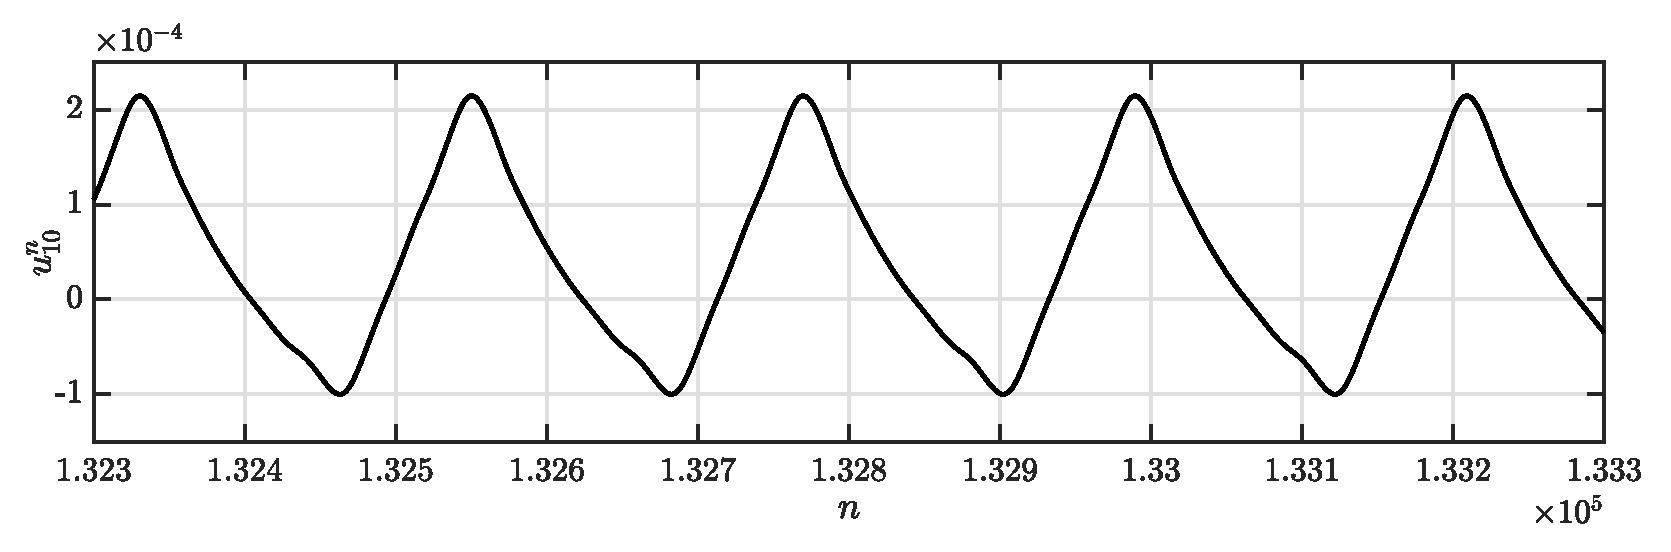
\includegraphics[width=\textwidth]{figures/exciters/elastoplasticWaveForm.eps}
    \caption{Time domain output at the bow location of a stiff string bowed using an elasto-plastic friction model. \label{fig:elastoWaveform}}
\end{figure}

\subsection{Stability through energy analysis}
As the elasto-plastic bow model is a differential equation in itself, its approximation will need to abide a stability condition as well.
As the system at hand is nonlinear, frequency domain analysis as described in Section \ref{sec:stabilityAnalysis} can not be performed. Energy analysis, on the other hand, can be used here to determine the necessary stability condition for this model. This section follows the concepts introduced in Section \ref{sec:stabilityAnalysisEnergy} to obtain a stability conditions for the elasto-plastic friction model. A similar process for finding stability for the LuGre model has been done by Olsson in continuous time \cite[p. 55]{Olsson1996}. The derivation below is inspired by his. 

First, all terms of Eq. \eqref{eq:elastoStiffStringFDS} are multiplied by $\rho A$ to get the appropriate units for the analysis. Then, the inner product with $\dtd \uln$ over the string domain $\D$ is taken to get
\begin{equation}
    \dtp \h_\text{s} + \q_\text{s} = -\p_\Btxt
\end{equation}
where the definitions for the discrete Hamiltonian $\h_\text{s}$ and the damping term $\q_\text{s}$ for the string can be found in Section \ref{sec:energyAnalysisString}. The input power introduced by the bow is defined as (writing $f(v^n,z^n) = f^n$)
\begin{equation*}
    \p_\Btxt = \langle (\dtd \uln), J(x_\Btxt^n)f^n\rangle_\D
\end{equation*}
which, using identity \eqref{eq:identityIJ} can be written as 
\begin{equation*}
    \p_\Btxt = I_l(x_\text{B}^n)\dtd \uln f^n.
\end{equation*}
Finally, using Eq. \eqref{eq:vrelElastoDisc} yields
\begin{equation}
    \p_\Btxt = f^nv^n + f^n v_\Btxt^n.
\end{equation}
The term $f^nv^n$ is the important one as $f^nv_\Btxt^n$ is a driving term, and is zero when the external bow velocity is zero. This means that this does not affect the internal stability of the system. In the following, the superscript $n$ is suppressed for brevity.

Substituting Eq. \eqref{eq:discForceFunction} into $fv$ and ignoring the noise term $s_3w^n$ for now, yields
\begin{equation}\label{eq:fv}
    \p_\Btxt = fv = \sigma_{0}zv +\sigma_{1}rv+\sigma_{2}v^2.
\end{equation}
The definition for $r^n$ in Eq. \eqref{eq:r} may be rewritten as
\begin{equation*}
    \begin{aligned}
        r &= v\bigg[1-\alpha\frac{z}{z_\text{ss}(v)}\bigg],\\
        r &= v-\frac{v\alpha z}{z_\text{ss}(v)},\\
        v &= r + \frac{v\alpha z}{z_\text{ss}(v)},
    \end{aligned}
\end{equation*}
and (following Olsson) may be substituted in Eq. \eqref{eq:fv} as
\begin{equation}
    \p_\Btxt = s_{0}z\left(r+ \frac{v\alpha z}{z_\text{ss}(v)}\right)+s_{1}r\left(r+ \frac{v\alpha z}{z_\text{ss}(v)}\right)+s_{2}v^2,
\end{equation}
or
\begin{equation}
    \p_\Btxt = s_0zr+s_1\left(r+\frac{v\alpha z}{2z_\text{ss}(v)}\right)^2+\frac{v\alpha z^2}{z_\text{ss}(v)}\left(s_0-\frac{s_1v\alpha}{4z_\text{ss}(v)}\right)+s_2v^2.
\end{equation}
The power introduced by the bow can then be subdivided into the total energy in the bristles and their damping. As $r$ approximates $\dot z$ the first term, one can rewrite this to 
\begin{equation*}
    \dtp \h_\text{brist} + \q_\text{brist} \geq 0,
\end{equation*}
and needs to be non-negative for passivity. 

Starting with the damping term, which is defined as
\begin{equation}
    \q_\text{brist} = s_1\left(r+\frac{v\alpha z}{2z_\text{ss}(v)}\right)^2+\frac{v\alpha z^2}{z_\text{ss}(v)}\left(s_0-\frac{s_1v\alpha}{4z_\text{ss}(v)}\right)+s_2v^2.
\end{equation}
one can show that, as all coefficients are non-negative and $\sgn(v) = \sgn(z_\text{ss}(v))$ (through a multiplication by $\sgn(v)$ in the definition of in Eq. \eqref{eq:zss}), $\q_\text{brist}$ is non-negative under the following condition:
\begin{equation}
    s_1 \leq \frac{4s_0z_\text{ss}(v)}{v}\ .
\end{equation}
This means that as long as one knows the limit of the velocity of the system, the coefficient $s_1$ can be set accordingly.

Using identity \eqref{eq:prodIdentity2}, the energy stored in the bristles can be shown to be
\begin{equation}
    \h_\text{brist} = \frac{s_0}{2}z^ne_{t-}z^n,
\end{equation}
which is not necessarily non-negative. In \cite{Olsson1996}, Olsson performs the analysis in continuous time, where the energy in the bristles is defined as to 
\begin{equation}
    \mathfrak{H}_\text{brist} = \frac{s_0}{2} z^2,
\end{equation}
which is clearly non-negative. See Notes below for a discussion. 

% A condition can, however, be retrieved from the damping term and is similar to the condition presented by Olsson in continuous time. The damping term is defined as

\subsubsection{\SWcomment[NOTES FOR STEFAN]}
As far as I see, to find a stability condition for the model, there are two options:
\begin{enumerate}
    \item The $s_0z$ term should be discretised using the centred averaging operator, such that the system is inherently stable.
    \begin{equation}
        s_0 (\mtd z^n)(\dtd z^n)\quad \overset{\text{Eq. \eqref{eq:prodIdentity4}}}{\Longrightarrow} \quad \frac{s_0}{2}\mtm(z^n)^2
    \end{equation}
    This introduces the issue of needing to deal with $z^{n+1}$ issue in the multivariate NR solve.. 
    \item If the bristles had some sort of mass, one could create a stability condition such as done for the mass-spring system in Section \ref{sec:stabilityAnalysisEnergy}. This requires a change the model.
    \item Or do you see something I don't...?
\end{enumerate}

\section{Discussion and conclusion}
This chapter presented the bow as a mechanism to excite stiff strings. Two friction models have been presented: a static friction model where the friction force is only a function of the relative velocity between the string and the bow, and a dynamic elasto-plastic friction model, which relates this relative velocity to the friction force using a differential equation. The latter has been presented in paper \citeP[C] where it was first applied to stiff strings based on FDTD methods. 

Although a successful implementation of the elasto-plastic friction model has been made, it has not been used in the project beyond paper \citeP[C]. It was found that small changes in parameters, both control and model parameters, already yield large behavioural changes. An attempt was made at using the elasto-plastic friction model with a fully modelled instrument (the tromba marina presented in papers \citeP[D] and \citeP[E]), but did not yield the desired results, and the predictable static friction model was chosen instead. Future work includes tuning the many parameters that the elasto-plastic model relies on and apply an adjusted version to fully modelled instruments.

An in-depth comparison between the static and the elasto-plastic friction model in terms of perceptual differences, is also left for future work. A preliminary comparison has been carried out by Onofrei in \cite{Onofrei2021}, where the author noted that \textit{"the
elasto-plastic model seems to behave more smoothly"} than the static friction model. This is also what is observed when comparing the output of the friction models in Figures \ref{fig:helmholtzImplementation} and \ref{fig:elastoWaveform}. As said, these observations are preliminary, and further work needs to be done to compare the various friction models.

Finally, it must be noted that the applications of the bow are not limited to strings, and can very well be extended to other resonators. In [\hyperref[ch:listOfPublications]{S4}], for example, the authors apply the elasto-plastic friction model to a 2D drum membrane to simulate a friction drum inspired instrument.